\begin{showExamples}%
%
%%%%%%%%%%%%%%%%%%%%%%%%%%%%%%%%%%%%%%%%%%%%%%%%%%%%%%%%%%%%
\chapter{Anleitung zur Nutzung dieser Vorlage}%
\label{chap:Examples}
%%%%%%%%%%%%%%%%%%%%%%%%%%%%%%%%%%%%%%%%%%%%%%%%%%%%%%%%%%%%
%
%
Dieses Kapitel, welches in anderen Kapiteln als \cref{chap:Examples} referenziert werden könnte, zeigt den grundlegenden Aufbau eines einfachen Kapitels.
Die einzelnen Abschnitte beschreiben die Struktur der Vorlage und geben wichtige allgemeine Tipps.
Die Verwendung einzelner Features dieser Vorlage wird in \cref{chap:Examples} detailliert beschrieben und demonstriert.

Es wird empfohlen, die einzelnen Unterkapiteln jedes Kapitels als eigene Dateien anzulegen und sie mit dem \verb+\input{}+-Befehl einzubinden (s. Quelltext).
Dies erlaubt die einzelnen Unterkapitel bei Bedarf leichter zu verschieben oder mit einem einzigen \%-Zeichen temporär auszukommentieren und erleichtert so die Fehlersuche.

Zur Nutzung dieser Vorlage für die eigene Arbeit empfiehlt es sich, die Anleitungskapiteln auszublenden und ansonsten die bestehende Struktur zu nutzen.
Die Anleitungskapiteln lassen sich ausblenden, indem man in der Hauptdatei \texttt{Diss.tex} in der Zeile 27 \verb+\showif{showExamples}+ durch \verb+\hideif{showExamples}+ ersetzt.%
%
\footnote{Die Befehle \verb+\showif{showExamples}+ bzw. \verb+\hideif{showExamples}+ definieren die Umgebung \texttt{showExamples}, deren Inhalt jeweils angezeigt bzw. ausgeblendet wird.
Dies betrifft alles, was zwischen \verb+\begin{showExamples}+ und \verb+\end{showExamples}+ steht.
Der Vorteil dieser Vorgehensweise gegenüber einem einfachen Auskommentieren liegt darin,
dass die zwischen \verb+\begin{showExamples}+ und \verb+\end{showExamples}+ eingebundenen Dateien
weiterhin im Verzeichnisbaum vom TeXnicCenter etc. sichtbar bleiben und bei Bedarf schnell aufgerufen werden können.}
%
Ähnlich lassen sich auch andere Teile des Manuskriptes ausblenden ohne sie auskommentieren zu müssen.
%
%%%%%%%%%%%%%%%%%%%%%%%%%%%%%%%%%%%%%%%%%%%%%%%%%%%%%%%%%%%%
\section{Kompilierung der Vorlage}%
\label{sec:Kompilierung}
%%%%%%%%%%%%%%%%%%%%%%%%%%%%%%%%%%%%%%%%%%%%%%%%%%%%%%%%%%%%
%
Um diese Vorlage nutzen zu können, benötigt man eine \LaTeX-Distribution (z.B. \printswname{MiKTeX}\footnote{\url{http://www.miktex.org/}} oder \printswname{TeXLive}\footnote{\url{https://tug.org/texlive/acquire.html}}).
Sofern man nicht die riesengroße Komplettinstallation wählt, wird beim ersten Kompilieren eine Internet"=Verbindung benötigt, um Zusatz"=\glspl{gls:pkg} dynamisch nachladen zu können.
Zur Erstellung des Glossars und des Abkürzungsverzeichnisses wird zusätzlich Perl benötigt.
Unter Windows müsste hierzu zusätzlich beispielsweise \printswname{ActivePerl}\footnote{\url{https://www.activestate.com/products/activeperl/}}
oder \printswname{StrawberryPerl}\footnote{\url{http://strawberryperl.com/}} installiert werden.
Bei den Linux-Distributionen ist Perl automatisch mit dabei.

Zur bequemen Bearbeitung der \LaTeX"=Quellcode"=Dateien empfiehlt sich Verwendung einer guten \LaTeX"=Entwicklungsumgebung in Kombination mit einem geeigneten, sprich SyncTeX"=fähigen, PDF"=Betrachter.
Manche Entwicklungsumgebungen bieten eine integrierte PDF"=Vorschau, welche Vor- und Nachteile haben kann.
Ein wichtiges Kriterium bei der Wahl der Entwicklungsumgebung ist die Möglichkeit, zwischen den einzelnen Stellen im Quellcode und im PDF hin- und her springen zu können.
Unter Windows war lange Zeit \textbf{TeXnicCenter}\footnote{\url{http://www.texniccenter.org/}} in Kombination mit \printswname{SumatraPDF}\footnote{\url{https://www.sumatrapdfreader.org}} eine gute Wahl gewesen.
Mittlerweile tendieren die meisten dazu, \printswname{TeXstudio}\footnote{\url{https://www.texstudio.org/}} zu verwenden.
Diese bietet eine eingebaute PDF"=Vorschau und viele nützliche Features und ist sowohl unter Windows als auch unter Linux verfügbar.

%%%%%%%%%%%%%%%%%%%%%%%%%%%%%%%%%%%%%%%%%%%%%%%%%%%%%%%%%%%%
\subsection{MiKTeX-Einstellungen}
\label{sec:MiKTeX}
%%%%%%%%%%%%%%%%%%%%%%%%%%%%%%%%%%%%%%%%%%%%%%%%%%%%%%%%%%%%
Sofern MiKTeX als \LaTeX"=Distribution verwendet wird, sollte man darauf achten, dass bei Bedarf Zusatzpakete vom Internet dynamisch nachgeladen werden können.
Sofern diese Option nicht bei der Installation gesetzt worden ist, kann sie nachträglich in der MiKTeX-Console aktiviert werden.
Zu finden ist diese im Startmenü unter \enquote{MiKTeX}, \enquote{MiKTeX Console (Admin)}.
Unter \enquote{Settings} findet sich ein Reiter \enquote{General}, wo im Bereich \enquote{Package installation} entweder die Option \enquote{Always install missing packages on the fly} oder \enquote{Ask me} ausgewählt werden soll.
Sofern sich der Rechner im Netzwerk des Fraunhofer IOSB befindet, muss zusätzlich noch die Proxy-Option korrekt gesetzt werden.
Hierfür muss man im Bereich \enquote{Package installation} der MiKTeX Console auf \enquote{Change} gehen und bei \enquote{Connection Settings} die Verwendung des Proxy-Servers \printkeyword{proxy-ka.iosb.fraunhofer.de} mit Port \printkeyword{80} aktivieren (s. \cref{fig:MiKTeX-Proxy}).
Wird dies nicht gemacht, können benötigte Pakete nicht nachgeladen werden.

\begin{figure}[htb]%
\centering%
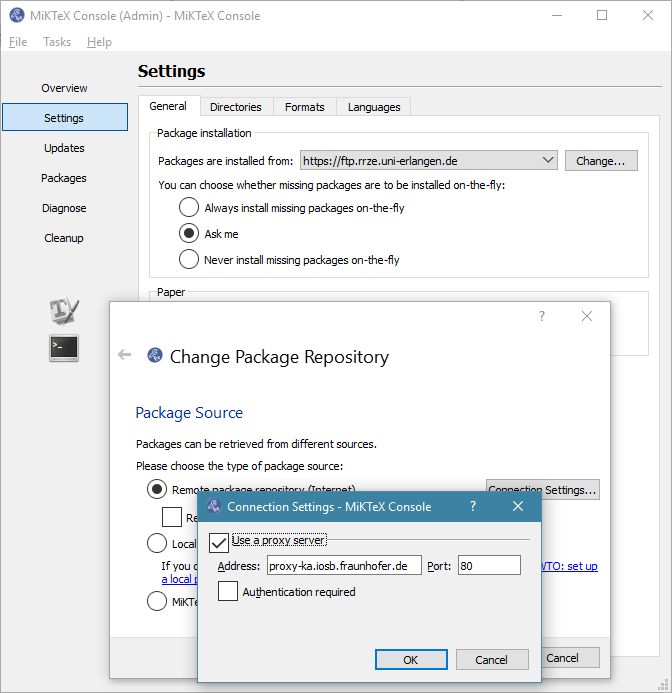
\includegraphics[width=\linewidth]{images/examples/MiKTeX-Proxy.png}%
\caption{MiKTeX-Einstellungen zum Nachladen der Zusatzpakete}%
\label{fig:MiKTeX-Proxy}%
\end{figure}

Nach der MiKTeX-Installation sollte man im Startmenü gleich die MiKTeX-Console aufrufen, den Proxy eintragen und das Update durchführen um die aktuellste Version der vorinstallierten Pakete zu erhalten.
So vermeidet man beim automatischen Nachladen weiterer \glspl{gls:pkg} aus dem \acrshort{ac:CTAN}-Repository etwaige Inkompatibilitäten aufgrund veralteter Stammpakete.


%%%%%%%%%%%%%%%%%%%%%%%%%%%%%%%%%%%%%%%%%%%%%%%%%%%%%%%%%%%%
\subsection{TeXLive-Einstellungen}
\label{sec:TeXLive}
%%%%%%%%%%%%%%%%%%%%%%%%%%%%%%%%%%%%%%%%%%%%%%%%%%%%%%%%%%%%
Bei Verwendung von TeXLive unter Linux muss darauf geachtet werden, dass alle notwendigen Linux-\glspl{gls:pkg} installiert sind.
Unter Ubuntu 17.04 sollte es funktionieren, wenn folgende Linux-\glspl{gls:pkg} installiert wurden:
\begin{itemize*}
	\item {\small\verb#texlive#}
	\item {\small\verb#texlive-lang-german#}
	\item {\small\verb#texlive-fonts-extra#}
	\item {\small\verb#texlive-bibtex-extra#}
	\item {\small\verb#fonts-linuxlibertine#}
	\item {\small\verb#biber#}
	\item {\small\verb#xindy#}
	\item {\small\verb#texmaker#}
\end{itemize*}
Texmaker ist eine IDE für \LaTeX, die aber vermutlich über Dependencies schon einige Pakete mitbringt.


%%%%%%%%%%%%%%%%%%%%%%%%%%%%%%%%%%%%%%%%%%%%%%%%%%%%%%%%%%%%
\subsection{Kompilieraufrufe}
\label{sec:Aufruf}
%%%%%%%%%%%%%%%%%%%%%%%%%%%%%%%%%%%%%%%%%%%%%%%%%%%%%%%%%%%%
Zur erfolgreichen Kompilierung des Dokumentes müssen mehrere
Kommandozeilenprogramme aufgerufen werden.
Bei Verwendung einer integrierten Entwicklungsumgebung (IDE),
wird diese so konfiguriert, dass die Aufrufe aus der IDE heraus erfolgen und
die etwaigen Warnungen, Erfolgs- und Fehlermeldungen in der IDE sichtbar werden.
Die entsprechenden Einstellungen für TeXnicCenter und TeXstudio finden sich
in den nachfolgenden Kapiteln.

Die einzelnen Aufrufe sind:
\begin{itemize*}
\item \index{xelatex}\texttt{xelatex} zur eigentlichen Kompilierung von \LaTeX-Quelltext,
\item \index{biber}\texttt{biber} zur Kompilierung von Bibliografien,
\item \index{makeglossaries}\texttt{makeglossaries}, welches intern \index{xindy}\texttt{xindy} aufruft,
zur Erstellung einer Zwischenausgabe für das Abkürzungsverzeichnis und das Glossar
\index{makexindex}\texttt{makeindex}, welches durch die Verwendung des Pakets \pkg{imakeidx} implizit aufgerufen wird, zur Erstellung des Stichwortverzeichnisses
\end{itemize*}
Bei einem Durchlauf von \texttt{xelatex}, \texttt{biber}, \texttt{makeglossaries} und \texttt{makeindex}
werden die einzelnen Inhalte sowie die entsprechenden Querverweise
zuerst jeweils in eine oder mehrere Zwischendateien hinausgeschrieben,
die sodann wieder eingelesen und verarbeitet werden müssen.
Manche Inhalte werden daher erst jeweils beim zweiten Aufruf von \texttt{xelatex} generiert.
Für die korrekte Generierung eines Dokumentes mit allen Verzeichnissen
(Inhalts-, Abbildungs-, Tabellen-, Literatur, Abkürzungs-, Begriffs und Stichwortverzeichnis),
PDF"=Lesezeichen und korrekt gesetzten Querverweisen,
muss \texttt{xelatex} daher mehrmals aufgerufen werden.

Sollte man ausnahmsweise das Dokument doch noch aus der Kommandozeile oder von einem Script heraus aufrufen wollen,
so ist die Reihenfolge der Aufrufe wie folgt:
\begin{verbatim}
#> xelatex -synctex=1 -interaction=nonstopmode Diss.tex
#> xelatex -synctex=1 -interaction=nonstopmode Diss.tex
#> biber Diss
#> makeglossaries Diss
#> xelatex -synctex=1 -interaction=nonstopmode Diss.tex
#> xelatex -synctex=1 -interaction=nonstopmode Diss.tex
\end{verbatim}

Wenn kein \index{Kompilierfehler}Kompilierfehler aufgetreten ist,
sollte nach dem vierten Durchlauf von \texttt{xelatex} die
\index{Warnung!Please re-run latex}Warnung \enquote{Please re-run latex}
verschwunden sein.
%%%%%%%%%%%%%%%%%%%%%%%%%%%%%%%%%%%%%%%%%%%%%%%%%%%%%%%%%%%%
\section{Aufbau der Vorlage}%
\label{sec:AufbauDerVorlage}
%%%%%%%%%%%%%%%%%%%%%%%%%%%%%%%%%%%%%%%%%%%%%%%%%%%%%%%%%%%%
%
Die Vorlage besteht aus mehreren Dateien und Verzeichnissen.
Ihre Bedeutung ist in \cref{tab:StrukturDerVorlage} zusammengefasst.
%
%{\footnotesize
\begin{table}[htbp]
%\scriptsize% kleinere Schrift
\footnotesize% kleinere Schrift
\centering%% Tabelle zentrieren (falls nicht volle Seitenbreite)
\renewcommand{\arraystretch}{1.5}% Abstand zwischen den Zeilen auf 1,5faches
\setlength{\tabcolsep}{0pt}% Seitliche Abstände eliminieren
% Tabelle auf die Seitenbreite strecken
\begin{tabularx}{\columnwidth}%
% Breite der ersten Spalte auf Inhalt anpassen,
% Breite der zweiten Spalte automatisch bestimmen,
%Spacing zwischen den Spalten auf 10pt setzen:
{l@{\extracolsep{8pt}}X}%
%-----------------------------------------------------------------------------------------------------
\toprule%
%-----------------------------------------------------------------------------------------------------
\bfseries Datei/Verzeichnis               & \bfseries Bedeutung und Benutzerinteraktion\\
%-----------------------------------------------------------------------------------------------------
\midrule%
%-----------------------------------------------------------------------------------------------------
\texttt{./Diss.tcp}                       & TeXnicCenter-Projektdatei. Aufruf im TeXnicCenter.
                                          Indirekte Änderung durch Einstellungen im Programm.\\
%-----------------------------------------------------------------------------------------------------
\texttt{./Diss.tex}                       & \texttt{TeX}-Hauptdatei. Aus- und Einblenden der einzelnen Manuskript-Teile
                                          durch Ersetzen von \lc{showif} durch \lc{hideif} und vice versa.\\
%-----------------------------------------------------------------------------------------------------
\texttt{./bib/Diss.bib}                   & Literaturdatenbank im \texttt{BibLaTeX}-Format. Verwendete Referenzen einfügen.\\
%-----------------------------------------------------------------------------------------------------
\texttt{./content/*}                      & Inhalte der Arbeit. Hier Inhalte der einzelnen \texttt{LaTeX}-Kapitel einfügen.\\
%-----------------------------------------------------------------------------------------------------
\texttt{./figures-src/*}                  & \texttt{TikZ}-Zeichnungen. %(Quellcode).
                                          Ggf. weitere hinzufügen.\\
%-----------------------------------------------------------------------------------------------------
\texttt{./figures-compiled/*}             & Temporäre Kompilate der \texttt{TikZ}-Zeichnungen.
                                          Bei Aktualisierung der \texttt{TikZ}-Zeichnungen löschen.\\
%-----------------------------------------------------------------------------------------------------
\texttt{./fonts/*}                        & Verwendete Schriften. Keine.\\
%-----------------------------------------------------------------------------------------------------
\texttt{./images/*}                       & Bilder im Binärformat. %(jpg, png, pdf etc).
                                          Ggf. weitere hinzufügen. \\
%-----------------------------------------------------------------------------------------------------
\texttt{./preambel/*}                     & Konfigurationsdateien. S.u.\\
%-----------------------------------------------------------------------------------------------------
\texttt{./preambel/Acronyms.tex}          & Definition der Akronyme.
                                          Ggf. weitere hinzufügen.\\
%-----------------------------------------------------------------------------------------------------
\texttt{./preambel/AlleAngaben.tex}       & Angaben zum Typ der Arbeit, zum Autor und zu den Gutachtern.
                                          Einstellung der Hauptsprache.\\
%-----------------------------------------------------------------------------------------------------
\texttt{./preambel/AllePfade.tex}         & Definition von Suchpfaden für Bildverzeichnisse und Bibliografie"=Dateien.
                                          Ggf. ergänzen.\\
%-----------------------------------------------------------------------------------------------------
%\texttt{./preambel/BibSettings.tex}       & Konfiguration der Bibliografie
%                                          Normalerweise keine, es sei denn man möchte den Stil der Literaturverzeichnisse ändern. \\
%-----------------------------------------------------------------------------------------------------
%\texttt{./preambel/EncodingAndFont.tex}   & Schriftarteinstellungen
%                                          Keine.\\
%-----------------------------------------------------------------------------------------------------
\texttt{./preambel/Glossary.tex}          & Definition der Glossar-Einträge.
                                          Ggf. weitere hinzufügen.\\
%-----------------------------------------------------------------------------------------------------
\texttt{./preambel/GlossarySymbols.tex}   & Glossar-Einträge für automatisches Symbolverzeichnis.
                                          Bei Verwendung ergänzen.\\
%-----------------------------------------------------------------------------------------------------
\texttt{./preambel/Header.tex}            & Alle Präambel-Definitionen (\teilw in weiteren Dateien).
                                          Aktivierung der \printkeyword{draft}-Option und des A4-Layouts.\\
%-----------------------------------------------------------------------------------------------------
\texttt{./preambel/Hyphenation.tex}       & Silbentrennung für unbekannte Wörter.
                                          Ggf. Regeln für die Silbentrennung weiterer Begriffe hinzufügen.\\
%-----------------------------------------------------------------------------------------------------
%\texttt{./preambel/IndexStyle.tex}        & Layout des Stichwortverzeichnisses.
%                                          Keine.\\
%-----------------------------------------------------------------------------------------------------
%\texttt{./preambel/KomaOptions.tex}       & KomaScript-Optionen.
%                                          Keine.\\
%-----------------------------------------------------------------------------------------------------
\texttt{./preambel/Math.tex}              & Mathe-Einstellungen und Makros.
                                          Bei Bedarf eigene Mathe-Makros definieren.\\
%-----------------------------------------------------------------------------------------------------
\texttt{./preambel/MyPackages.tex}        & Zusatzpakete
                                          Ggf. Einbindung von Zusatzpaketen.\\
%-----------------------------------------------------------------------------------------------------
\texttt{./preambel/Newcommands.tex}       & Eigene \LaTeX{}-Makros.
                                          Ggf. weitere Makros hinzufügen.\\
%-----------------------------------------------------------------------------------------------------
%\texttt{./preambel/preambel-commands.tex} & Paketkonfigurationen.
%                                          Normalerweise keine.\\
%-----------------------------------------------------------------------------------------------------
%\texttt{./preambel/settings.tex}          & Einstellungen zu Längen, Breiten, Verzeichnistiefen etc.
%                                          Normalerweise keine.\\
%-----------------------------------------------------------------------------------------------------
%\texttt{./preambel/TableCommands.tex}     & Tabelleneinstellungen.
%                                          Normalerweise keine.\\
%-----------------------------------------------------------------------------------------------------
%\texttt{./preamble/Translations.tex}      & Multilinguale Begriffsdefinitionen.
%                                          Normalerweise keine.\\
%-----------------------------------------------------------------------------------------------------
\bottomrule%
%-----------------------------------------------------------------------------------------------------
\end{tabularx}%
\caption[Dateien und Verzeichnisse der Vorlage]{Dateien und Verzeichnisse der Vorlage}%
\label{tab:StrukturDerVorlage}%
\end{table}

Bei der Datei \printfilepath{Diss.tcp} handelt es sich um die Projektdatei für den \LaTeX-Editor TeXnicCenter.
In ihr werden die projektbezogenen Einstellungen des TeXnicCenter festgehalten.
Das sind u.a. Angaben zur Hauptdatei des Projektes und zur Projektsprache.
Die korrekte Angabe der Projektsprache ist insofern wichtig, als dass diese in TeXnicCenter ab Version 2.0 Beta 1 zur Bestimmung der Sprache für die Rechtschreibprüfung verwendet wird.
Die entsprechenden Einstellungen können im TeXnicCenter über den Menüeintrag \printkeyword{Projekt} $\rightarrow$ \printkeyword{Eigenschaften} vorgenommen werden.


Die Hauptdatei ist die Datei \printfilepath{Diss.tex}.
Sie ist verhältnismäßig kurz, da die Hauptinhalte in andere Dateien ausgelagert sind, welche mit Hilfe des \lc{input\{\}} \bzw des \lc{include\{\}}-Befehls eingebunden werden.
Die Hauptdatei besteht im Wesentlichen aus vier Abschnitten.
Im ersten stehen die sogenannten \enquote{Magic comments}, mit deren Hilfe manche \LaTeX-IDEs sich selbst vorkonfigurieren können.
Sie fangen mit \enquote{\texttt{\%~!TeX}} an und geben an, welche Kodierung für die Dateien verwendet wird und welche Programme für die Kompilierung des Quelltextes und der Bibliografie verwendet werden sollen.
Außerdem kann hier angegeben werden, welche Sprache für die Rechtschreibprüfung innerhalb der IDE verwendet werden soll.
Im zweiten Abschnitt wird die Header-Datei eingebunden.
In dieser wird die verwendeten Dokumentklasse (inklusive Papierformat und Schriftgröße) definiert, sowie weitere Dateien eingebunden,
in welchen die zu landenden Pakete, Layout"=Parameter sowie alle weiteren Einstellungen definiert und konfiguriert werden.
Im dritten Teil können mit Hilfe von Schaltern einzelne Teile der Arbeit aus- und wieder eingeblendet werden, ohne dass sie auskommentiert werden müssen.
Im vierten Teil werden nun die einzelnen Inhalte der Arbeit eingebunden.

Das entstehende PDF heißt genauso wie die Hauptdatei.

Die einzelnen \index{Kapitel}Kapiteln der Arbeit werden im Verzeichnis \printfilepath{./content/} als separate Dateien gespeichert.
Es empfiehlt sich als Dateiname das Schema \printfilepath{nn-name.tex} zu verwenden, wobei \printkeyword{nn} die Nummer des Kapitels ist,
sodass die Dateien in der semantisch richtigen Reihenfolge sortiert angezeigt werden.
Die einzelnen Dateien werden per \verb+include{}+-Direktive in der Datei \printfilepath{Diss.tex} eingebunden.
Theoretisch wäre es an dieser Stelle auch möglich mit \verb+\input{}+ zu arbeiten, was jedoch seine Nachteile hätte.
Der Unterschied zwischen den beiden Befehlen wird \href{https://texwelt.de/wissen/fragen/32/was-ist-der-unterschied-zwischen-include-and-input}{auf texwelt.de} erklärt:

\begin{quote}
{\small
\verb+\input{file}+ lädt die Datei an Ort und Stelle in die Ziel-Datei und ist äquivalent
als ob man den Text in \printkeyword{file} direkt in die Ziel-Datei geschrieben hätte.
\verb+\input+ kann letztlich überall für jede Art Datei verwendet werden und kann auch verschachtelt angewendet werden,
d.h. eine eingebundene Datei kann ihrerseits Dateien mit \verb+\input+ einbinden.

\verb+\include{file}+ hingegen führt zunächst einmal ein \verb+\clearpage+ aus bevor es \verb+\input{file}+ ausführt.
Im Gegensatz zu \verb+\input+ kann eine Datei, die mit \verb+\include+ eingebunden wird,
kein weiteres \verb+\include+ enthalten, es ist also keine verschachtelte Anwendung möglich.
Eine mit \verb+\include+ eingebundene Datei kann aber natürlich \verb+\input+ enthalten.
\verb+\include+ erzeugt eine neue \printfilepath{aux}-Datei für die eingebundene Datei.
Das erlaubt es beispielsweise, ein Dokument in mehrere logische Einheiten zu zerlegen (etwa einzelne Kapitel),
die jede einer Datei entsprechen, die mit \verb+\include+ in die Hauptdatei eingebunden wird.
\verb+\includeonly{file1,file3}+ würde dann erlauben, nur gerade bearbeitete Dateien für die Kompilation einzubinden
und durch die separaten \printfilepath{aux}-Dateien dennoch korrekte Seitenzahlen und Querverweise zu erhalten.
Es gibt auch das \pkg{excludeonly} Paket, dessen Befehl \verb+\excludeonly+ das gegensätzliche Verhalten bietet.%
}%
\footnote{\url{https://texwelt.de/wissen/fragen/32/was-ist-der-unterschied-zwischen-include-and-input}}
\end{quote}

Zur besseren Übersicht und zur Vereinfachung der Fehlersuche wird empfohlen,
die einzelnen Unterkapitel ebenfalls als separate Dateien in Unterverzeichnissen von \printfilepath{./content/} anzulegen
und sie mit den \verb+\input{}+-Direktiven in die jeweiligen Kapitel-Dateien einzubinden.

Es wird davon ausgegangen, dass sich sämtliche Bibliografie-Angaben in der Datei
\printfilepath{./bib/Diss.bib} befinden.
Sollten mehrere Bibliografie-Dateien verwendet werden, können diese in der Datei
\printfilepath{./preamble/AllePfade.tex} gesetzt werden.

\index{Bild}Bilder bzw. \index{Zeichnung|see{Bild}}Zeichnungen werden auf zwei Arten eingebunden.
Bilder im \index{Bild!Binär-}Binärformat (PNG, JPEG, TIFF, PDF, etc.)
werden mit \lc{includegraphics}-Befehl eingebunden. 
Bei den \index{Bild!TikZ}\gls{gls:tikz}-Zeichnungen handelt es sich um reguläre TeX-Quellcode-Dateien,
die mit dem \verb+\input+-Befehl eingebunden werden.
Für eine einfache Verwaltung wird empfohlen, Binärbilder im Verzeichnis \printfilepath{./images/} abzulegen.
Zusätzliche Pfade können in der Datei \printfilepath{./preambel/AllePfade.tex} definiert werden.
Die \gls{gls:tikz}-Quellcode-Dateien sollten im Verzeichnis \printfilepath{./figures-src/} abgelegt werden.
Während des Kompilierens werden für jede \gls{gls:tikz}-Zeichnung im Verzeichnis \printfilepath{./figures-compiled/} mehrere Dateien erzeugt.
Der Inhalt dieses Verzeichnisses kann gefahrlos gelöscht werden.
Weitere Hinweise und Beispiele zur Einbindung von Grafiken finden sich in \cref{sec:Bilder}.

Die wichtigsten Einstellungen, die auf jeden Fall geändert werden müssen,
finden sich in der Datei \printfilepath{./preambel/AlleAngaben.tex}.
Hier werden \ua Angaben zum Verfasser, Art und Titel der Arbeit sowie zu den Gutachtern gemacht.
Außerdem wird hier die Hauptsprache der Arbeit gesetzt, was sich an mehreren Stellen auswirkt.
So wird beispielsweise bei Umstellung auf Englisch als Hauptsprache
\enquote{Danksagung} durch \enquote{Acknowledgments},
\enquote{Inhaltsverzeichnis} durch \enquote{Contents}
\usw ersetzt.
Auch die Regeln der Silbentrennung werden entsprechend angepasst.

Regeln zur Silbentrennung unbekannter Wörtern (\zB von Fachbegriffen)
können in der Datei \printfilepath{./preambel/Hyphenation.tex} festgelegt werden.
Zu beachten ist, dass zusammengesetzte Wörter mit einem Bindestrich
ausschließlich am Bindestrich getrennt werden,
wogegen auch ein Eintrag in die Datei \printfilepath{Hyphenation.tex} nicht hilft.
Um Silbentrennung an anderen Stellen eines zusammengesetzten Wortes zu erlauben,
muss man den Bindestrich durch „\verb+"=+“ ersetzen%
\footnote{\url{https://de.wikibooks.org/wiki/LaTeX-W%C3%B6rterbuch:_Silbentrennung}}.

%%%%%%%%%%%%%%%%%%%%%%%%%%%%%%%%%%%%%%%%%%%%%%%%%%%%%%%%%%%%
\section[Grundsätzliches]{Grundsätzliches}%
\label{sec:Grundsätzliches}
%%%%%%%%%%%%%%%%%%%%%%%%%%%%%%%%%%%%%%%%%%%%%%%%%%%%%%%%%%%%
%
Beim Erstellen neuer Dateien bzw. Öffnen und Speichern bereits vorhandener Dateien ist darauf zu achten,
dass stets \index{UTF8-Kodierung}UTF-8 als Zeichenkodierung verwendet wird.
Wichtig ist dabei, dass alle tex-Dateien die UTF8-Kodierung ohne BOM haben,
worauf beim Anlegen neuer TeX-Dateien besonders zu achten ist
(am besten man kopiert und bearbeitet eine bereits vorhandene Datei).

Dank geeigneter Einstellungen in den Header-Dateien können deutsche Umlaute wie 
\index{Umlaute}%
ä,ö,ü,ß, Zeichen mit Akzent wie é sowie weitere UTF8-Zeichen wie z.B.
\index{Anführungszeichen}%
\index{Sprache!unterschiedliche Anführungszeichen}%
„deutsche“, “englische”, »französische« oder «russische» Anführungszeichen 
direkt im Quellcode eingegeben werden ohne irgendwelche Umwege wie z.B. 
\verb+"a+ für ä,
\verb+"u+ für ü,
\verb+\ss+, für ß und
\verb+'e+ für é.
Dies gilt insbesondere auch für Quellen des Literaturverzeichnisses (Bib-Dateien).

Die Zeiten, in welchen man sich bei der Eingabe deutscher Buchstaben verkünsteln musste,
sind zum Glück endgültig vorbei.

\myexcl{Wichtig!}
Normale, gerade Anführungszeichen (\texttt{{\dq}}) haben eine Sonderfunktion und sollten im Quellcode (außer in Listings) nicht verwendet werden.
Für die Eingabe von Anführungszeichen sollte man am besten die entsprechende Textstelle mit dem \lc{enquote\{...\}}"=Befehl umschließen.
Damit werden je nach Spracheinstellung des Dokumentes automatisch die richtigen Anführungszeichen gesetzt.
Außerdem werden so auch die \enquote{verschachtelten \enquote{Anführungszeichen}} korrekt behandelt.

Es empfiehlt sich, die einzelnen Sätze jeweils in einer neuen Zeile anzufangen.
Ein einfaches Zeilenumbruch wird von LaTeX wie ein Leerzeichen gehandhabt
und hat somit keinen Einfluss auf die Zeilenumbrüche im Ergebnisdokument.
Beim Rückwärtsspringen aus der PDF-Datei zum Quellcode wird dadurch jedoch
eine wesentlich bessere Lokalisierung der betroffenen Textstelle ermöglicht.
%%%%%%%%%%%%%%%%%%%%%%%%%%%%%%%%%%%%%%%%%%%%%%%%%%%%%%%%%%%%
\section[% Kurzversion für das Inhaltsverz., Kolumnentitel und PDF-Lesezeichen:
         Wichtiges zu Umbrüchen bei Überschriften
         \mbox{(Kurzversion für das Inhaltsverzeichnis etc.)}%
				]{% Langversion, die im Text gedruckt wird:
         Wichtiges zu Umbrüchen bei Überschriften
         (und ein Beispiel \newline für eine lange Überschrift,
         welche \newline für das Inhaltsverzeichnis und 
         \newline die Kolumnentiteln zu lang ist).%
				}%
\index{Zeilenumbruch}\index{Titel}\index{Überschrift}\index{PDF!Lesezeichen}%
\label{chap:Titles}
%%%%%%%%%%%%%%%%%%%%%%%%%%%%%%%%%%%%%%%%%%%%%%%%%%%%%%%%%%%%
%
%
Bei den Kapitelüberschriften kann man zwei Versionen definieren:
eine lange Überschrift in geschweiften Klammern, welche in der Arbeit selbst angezeigt wird, 
und optional eine Kurzversion in eckigen Klammern, welche im Inhaltsverzeichnis und in den 
\href{https://de.wikipedia.org/wiki/Kolumnentitel}{Kolumnentiteln}%
\footnote{Kolumnentitel sind Überschriften der einzelnen Seiten. Meist stehen sie in der Kopfzeile.}
angezeigt wird:
\begin{latex}
\section[Kurzversion]{Langer Titel}
\end{latex}
Dasselbe gilt für Bild- und Tabellenunterschriften. Hier kann man dem
\lc{caption}-Befehl ebenfalls einen optionalen Parameter übergeben.

Manchmal sind dem \glsdat{ac:KSP} die von \LaTeX{} automatisch eingefügten Zeilenumbrüche in den Kapitelüberschriften im Inhaltsverzeichnis nicht \enquote{schön} genug.
Ein manuelles Einfügen der Zeilenumbrüche etwa mit \verb+\newline+ in der Kurzversion des Titels funktioniert leider nicht,
da diese dann nicht nur im Inhaltsverzeichnis, sondern auch in den Kolumnentiteln und PDF"=Lesezeichen zur Geltung kommen, 
was normalerweise nicht erwünscht ist.

Abhilfe schafft der folgende Trick:
man schließt den letzten, umzubrechenden Teil der Kurzversion des Titels in eine \verb+\mbox{}+.
Der Text, der in eine \verb+\mbox{}+ eingeschlossen wird, darf nicht umbrochen werden.
Im Kolumnentiteln und in den PDF"=Lesezeichen hat dies keine besondere Wirkung; im Inhaltsverzeichnis führt dies jedoch dazu, dass \LaTeX{} den Zeilenumbruch vor der \verb+\mbox{}+ einfügt.
Dasselbe gilt für die ungünstig umbrochene Wörter (so will 
Ein entsprechendes Beispiel stellt die Überschrift dieses Abschnitts dar.
%%%%%%%%%%%%%%%%%%%%%%%%%%%%%%%%%%%%%%%%%%%%%%%%%%%%%%%%%%%%
\section[Bilder, Grafiken und Diagramme]{Bilder, Grafiken und Diagramme}
\label{sec:Bilder}
%%%%%%%%%%%%%%%%%%%%%%%%%%%%%%%%%%%%%%%%%%%%%%%%%%%%%%%%%%%%
%
Bei Einbindung von Grafiken sind zwei Fälle zu unterscheiden:
\begin{itemize*}
  \item reguläre \index{Bild!Binär-}Bilder in einem Binärformat
	      (\texttt{PNG}, \texttt{TIFF}, \texttt{JPG}, \texttt{PDF}, etc.)
	\item \index{Bild!Vektor-}Grafiken, die im \gls{gls:tikz}-Quellcode vorliegen 
\end{itemize*}

Grundlegender Unterschied bei der Einbindung \enquote{regulärer} Bilder
und \gls{gls:tikz}-Bilder ist, dass Binärformatgrafiken mit \lc{includegraphics\{...\}}
eingebunden werden, während \gls{gls:tikz}-Grafiken mit \lc{input\{...\}} eingebunden
und von \texttt{latex} mitkompiliert werden.


%%%%%%%%%%%%%%%%%%%%%%%%%%%%%%%%%%%%%%%%%%%%%%%%%%%%%%%%%%%%
\subsection[Floats]{\index{Float}\index{Bild!Float}Floats}%
\label{sec:Floats}
%%%%%%%%%%%%%%%%%%%%%%%%%%%%%%%%%%%%%%%%%%%%%%%%%%%%%%%%%%%%
%
Üblicherweise werden Bilder und Tabellen in Fließumgebungen (floats) gesetzt,
damit \LaTeX\ sie geschickt positionieren kann.
Bei Bildern heißt die entsprechende Float-Umgebung \printkeyword{figure}.
Die Positionierung kann durch Angabe von Buchstaben
\printkeyword{h}, \printkeyword{t}, \printkeyword{b} und \printkeyword{p}
beeinflusst werden
(\enquote{here}, \enquote{top}, \enquote{bottom}, \enquote{extra page}).

\myexcl{Wichtig!}
Seitens des \glsgen{ac:KSP} wird bezüglich Einbindung von Floats gefordert,
dass diese die einzelnen Sätze nicht zerreißen.
Dies bedeutet, dass eine Platzierung von Bildern und Tabellen lediglich
zwischen zwei Absätzen in Frage kommt.
Allerdings kann es passieren, dass der Platz auf der Seite nicht mehr ausreicht,
und das Bild nicht an der gewünschten Stelle gesetzt werden kann.
Damit wird das Bild auf die nächste Seite verschoben.
Bei aktivierter \printkeyword{t}- oder \printkeyword{b}-Option würde \LaTeX{} versuchen,
das Bild am oberen oder unteren Rand der Seite zu platzieren.
Allerdings passiert das dann häufig mitten in einem Satz,
was vom \gls{ac:KSP} ausdrücklich nicht erwünscht ist.
Somit bleibt eigentlich nur noch die Verwendung der \printkeyword{h}-Option.

Leider können dabei einige unerwünschte Effekte auftreten.
So können beispielsweise auf der vorherigen Seite riesige leere Flächen entstehen.
Wenn der verbleibende Platz auf der Seite eine Platzierung nicht erlaubt,
kann es schnell passieren, dass \LaTeX{} das betroffene Bild 
und alle Folgeilder ans Ende des Kapitels verschiebt
(genauer gesagt, an die Stelle, wo die nächste \lc{clearpage}-Anweisung kommt).

Eine genaue Auswirkung der Parameter
\printkeyword{h}, \printkeyword{t}, \printkeyword{b} und \printkeyword{p}
auf die Bildplatzierung ist nicht immer intuitiv.
Um diese zu verstehen, empfiehlt sich die Lektüre der Beschreibung
von Frank Mittelbach
\href{https://tex.stackexchange.com/questions/39017/how-to-influence-the-position-of-float-environments-like-figure-and-table-in-lat/39020#39020}{auf stackexchange.com}.%
\footnote{\url{https://tex.stackexchange.com/questions/39017/how-to-influence-the-position-of-float-environments-like-figure-and-table-in-lat/39020#39020}}

Prinzipiell empfiehlt sich eine endgültige Platzierung der Bilder erst ganz am Schluss,
nachdem alle anderen Korrekturen durchgeführt sind.
Ggf. müssen die Bilderdefinitionen manuell im Quellcode herumgeschoben werden,
bis die Abbildungen von \LaTeX\ optimal gesetzt werden.
Dafür empfiehlt es sich, die einzelnen Bilddefinitionen in Extra-Dateien auszulagern,
so dass nur noch eine einzige Zeile herumgeschoben werden muss.

%%%%%%%%%%%%%%%%%%%%%%%%%%%%%%%%%%%%%%%%%%%%%%%%%%%%%%%%%%%%
\subsection[Binärbilder]{\index{Bild!Binär-}Binärbilder}%
\label{sec:Binaerbilder}
%%%%%%%%%%%%%%%%%%%%%%%%%%%%%%%%%%%%%%%%%%%%%%%%%%%%%%%%%%%%
%
Ein Beispiel für die Einbindung eines Bildes im Binärformat ist in \cref{lst:binary-image} angeführt:

\begin{latex}[caption={Einbindung einer Binärgrafik in LaTeX},label={lst:binary-image}]
\begin{figure}[h]%
  \centering%
  \includegraphics[width=\linewidth]{Bildpfad/Dateiname}%
  \caption[Kurzversion für das Abbildungsverzeichnis]{%
           Eine tolle sehr lange Abbildungsunterschrift}%
  \label{fig:my-binary-image}%
\end{figure}
\end{latex}

Die Angabe des Pfades kann sowohl absolut als auch relativ
zum Verzeichnis der Hauptdatei oder zu einem der Pfade angegeben werden,
die in der Datei \printfilepath{./preambel/AllePfade.tex} definiert sind.
Diese Pfade werden in angegebenen Reihenfolge durchsucht.
Dasselbe gilt für die Dateierweiterung.
Ist keine Erweiterung definiert und liegen mehrere Bilder mit gleichem Namen jedoch unterschiedlicher Dateierweiterung vor,
wird die Reihenfolge, die in der Datei texttt{AllePfade.tex} definiert ist, verwendet.

Zu beachten ist dabei, dass der \gls{ac:KSP} Skalierung der Bildern auf die Seitenbreite fordert,
was hier durch die Option \printkeyword{width=\bs linewidth} verwirklicht wurde.

Wichtig anzumerken ist, dass alle Zeilen innerhalb der \printkeyword{Figure}"=Umgebung
mit einem Prozentzeichen abzuschließen sind.
Ansonsten werden überflüssige Leerzeichen eingefügt,
was zu unerwünschten Nebenwirkungen führen kann.

Mit Hilfe von Paket \pkg{subfig} \cite{Cochran2005} können Bilder auch in
\index{Abbildung|see{Bild}}\index{Bild!Unterabbildung}Unterabbildungen gesetzt
und sowohl als ganzes (vgl. \cref{fig:subfloat-example}) als auch einzeln (vgl.
\cref{fig:subfloat-example-01,fig:subfloat-example-02,fig:subfloat-example-03,fig:subfloat-example-04})
referenziert werden.

\begin{figure}[h]%
	\centering%
	\subfloat[La Savoureuse, Lepuix, Frankreich (\copyright\ Thomas Bresson)]{%
		\label{fig:subfloat-example-01}%
		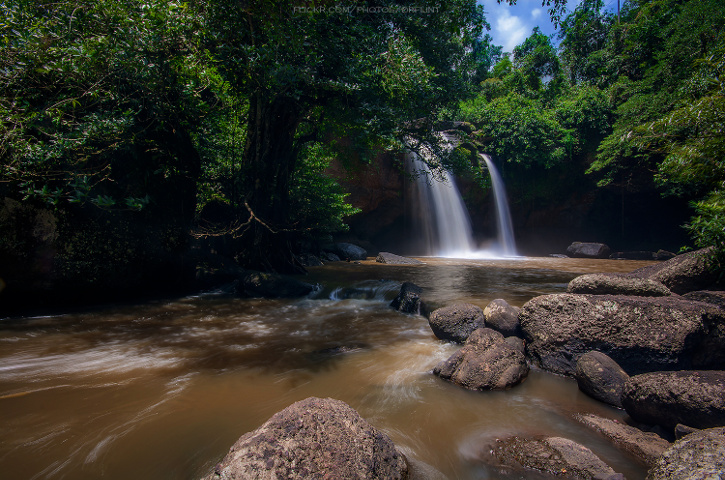
\includegraphics[width=0.49\linewidth]{./images/examples/subfloat-example-01.jpg}%
	}%
	\hfill%
	\subfloat[Bangkok, Thailand (\copyright\ Prachanart Viriyaraks)]{%
		\label{fig:subfloat-example-02}%
		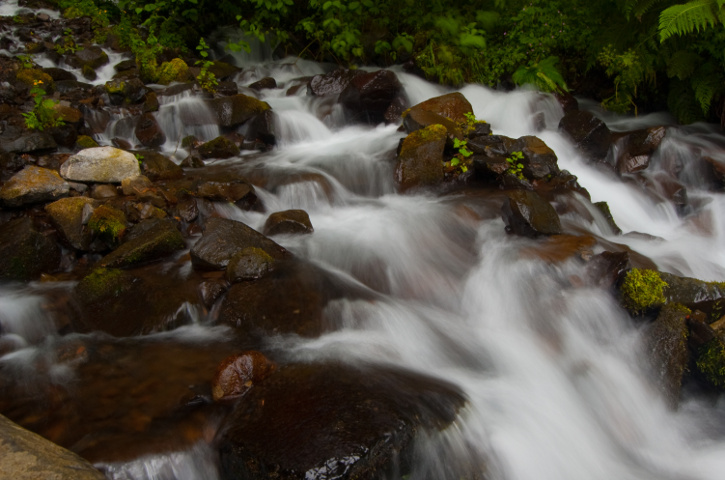
\includegraphics[width=0.49\linewidth]{./images/examples/subfloat-example-02.jpg}%
	}%
	\\%
	\subfloat[Wahkeena Falls, Lincoln Park, USA (\copyright\ srslyguys)]{%
		\label{fig:subfloat-example-03}%
		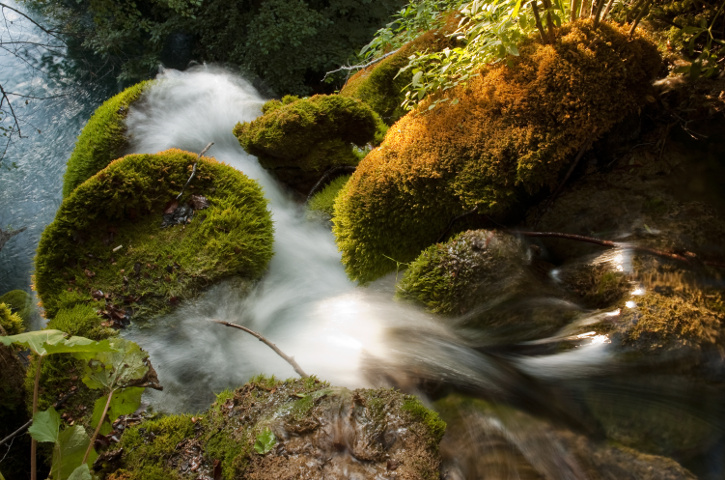
\includegraphics[width=0.49\linewidth]{./images/examples/subfloat-example-03.jpg}%
	}%
	\hfill%
	\subfloat[Nacionalni park Plitvička jezer, Kroatien (\copyright\ Roman Bonnefoy)]{%
		\label{fig:subfloat-example-04}%
		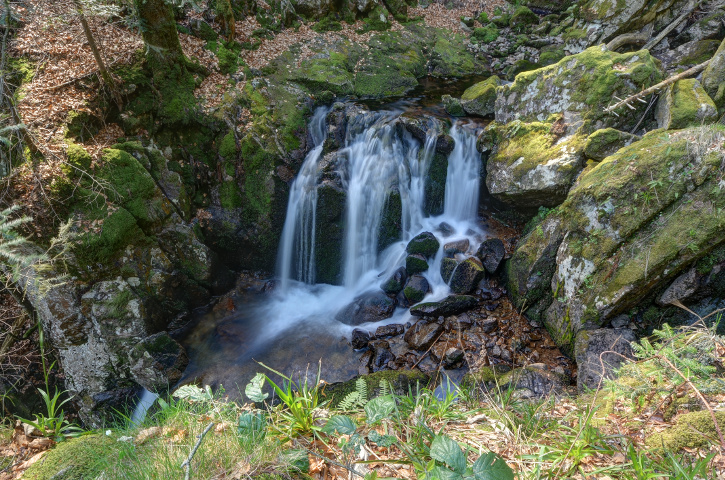
\includegraphics[width=0.49\linewidth]{./images/examples/subfloat-example-04.jpg}%
	}%
	\caption[Bild mit Unterabbildungen]{Wasserfälle der Welt als Beispiel für Unterabbildungen}%
	\label{fig:subfloat-example}%
\end{figure}

Der Beispielcode dafür ist in \cref{lst:subfigures} dargestellt.

\begin{latex}[caption={Unterabbildungen in LaTeX},label={lst:subfigures}]
\begin{figure}[h]%
	\centering%
	\subfloat[Unterbezeichnung 1)]{%
		\label{fig:UnterAbb1}%
		\includegraphics[width=0.49\linewidth]{Bildpfad/Bild1}%
	}%
	\hfill%
	\subfloat[Unterbezeichnung 2]{%
		\label{fig:UnterAbb2}%
		\includegraphics[width=0.49\linewidth]{Bildpfad/Bild2}%
	}%
	\\%
	\subfloat[Unterbezeichnung 3)]{%
		\label{fig:UnterAbb3}%
		\includegraphics[width=0.49\linewidth]{Bildpfad/Bild3}%
	}%
	\hfill%
	\subfloat[Unterbezeichnung 4]{%
		\label{UnterAbb4}%
		\includegraphics[width=0.49\linewidth]{Bildpfad/Bild4}%
	}%
\caption[Kurzversion]{Langversion der Bildunterschrift}%
\label{fig:MeinGanzesBild}%
\end{figure}
\end{latex}

Man beachte die abschließenden Prozent-Zeichen am Ende jeder Zeile!

%%%%%%%%%%%%%%%%%%%%%%%%%%%%%%%%%%%%%%%%%%%%%%%%%%%%%%%%%%%%
\subsection[TikZ-Grafiken]{\index{TikZ}\index{Bild!TikZ}\gls{gls:tikz}-Grafiken}%
\label{sec:TikZ}
%%%%%%%%%%%%%%%%%%%%%%%%%%%%%%%%%%%%%%%%%%%%%%%%%%%%%%%%%%%%
%
\Gls{gls:tikz} eignet sich hervorragend, um wissenschaftliche Zeichnungen,
Vektorgrafiken und \index{Diagramm}Diagramme direkt mithilfe von LaTeX
zu setzen, sodass die Schrift direkt zum restlichen Dokument passt.
Zu dem \pkg{tikz}-\gls{gls:pkg} und dem darauf aufsetzenden \pkg{PGFplots}-\gls{gls:pkg} gibt
es hervorragende Dokumentation \parencites{Tantau2013}{Feuersaenger2014}.
Mit \gls{gls:tikz} und \gls{gls:pgfplots} lassen sich viele gute Sachen machen.


Der Code für die Einbindung einer \gls{gls:tikz}-Grafik sieht folgendermaßen aus:
\begin{latex}[caption={Einbindung einer TikZ-Zeichnung in LaTeX},label={lst:tikz-figure}]
\begin{figure}[h]%
  \centering%
  \tikzsetnextfilename{TikZ-Bild}%
  \resizebox{\textwidth}{!}{%   <--- optionale Skalierung
    \input{./figures-src/TikZ-Bild.tex}%
  }%                            <--- optionale Skalierung
  \caption[Kurzversion für das Abbildungsverzeichnis]{%
           Eine tolle sehr lange Abbildungsunterschrift}%
  \label{fig:my-tikz-figure}%
\end{figure}
\end{latex}

Eine Skalierung auf die volle Seitenbreite oder ein vielfaches davon im Falle von Unterabbildungen kann bei Bedarf mit Hilfe der Anweisung
\texttt{\bs resizebox\{\bs textwidth\}\{!\}\{...\}}
durchgeführt werden.

Das Kommando \verb+\tikzsetnextfilename{...}+ ist nicht unbedingt notwendig,
 aber sehr zu empfehlen, da dies als Name für das temporäre Kompilat im Ordner
\printfilepath{./figures-compiled/} genommen wird.
Dieser sollte gleich dem Namen des Quelldatei (ohne Endung) gewählt werden.
Ansonsten nimmt \texttt{pdflatex} eine hochlaufende Nummer als Dateiname,
was die Fehlersuche sehr erschwert.

Nachfolgend finden sich einige Beispiele für TikZ-Zeichnungen, nämlich
eine Übersicht über die KIT-Corporate-Identity-Farben (\cref{fig:kit-colors}),
ein kommutatives Diagramm (\cref{fig:kpca}),
ein Netzwerkkommunikationsgraph (\cref{fig:net-comm}),
einfache \index{Diagramm!Punkt-}Punktdiagramme (\cref{fig:ica})
und etwas aufwendigere Diagramme mit mehreren
\index{Achsensystem|see{Diagramm}}Achsensystemen (\cref{fig:pca}).

Vorzugsweise sollten für die Grafiken die KIT-Corporate-Identity-Farben verwendet werden,
die sowohl eine RGB"=Definition für die Darstellung online,
als auch eine CMYK"=Definition für den Offset-Druck haben.%
\footnote{Bei Erstellung der Manuskriptversionen
für die Online-Veröffentlichung bzw. für den Offset-Druck
ist auf die korrekte Einstellung der Option \printkeyword{useCMYKcolors}
in der Datei \printfilepath{preambel/AlleAngaben.tex} zu achten
(\printkeyword{false} für die Online-Veröffentlichung und \printkeyword{true} für den Druck!}

\begin{figure}[hp]%
	\centering%
  \tikzsetnextfilename{kit-colors}%
	%\resizebox{\textwidth}{!}{%
		\begin{tikzpicture}[
box/.append style={rectangle,inner sep=0pt,outer sep=0pt,minimum size=1.5em,draw=none,fill=#1},
label/.style={font={\ttfamily\footnotesize},anchor=east},
caption/.style={font={\ttfamily\footnotesize},rotate=90,anchor=west}
]
\matrix[row sep=.2em,column sep=.2em] {
  &
\node[caption] {\textbackslash{}KITgreen...};      &
\node[caption] {\textbackslash{}KITblue...};       &
\node[caption] {\textbackslash{}KITblack...};      &
\node[caption] {\textbackslash{}KITpalegreen...};  &
\node[caption] {\textbackslash{}KITyellow...};     &
\node[caption] {\textbackslash{}KITorange...};     &
\node[caption] {\textbackslash{}KITbrown...};      &
\node[caption] {\textbackslash{}KITred...};        &
\node[caption] {\textbackslash{}KITlilac...};      &
\node[caption] {\textbackslash{}KITcyanblue...};   \\
\node[label] {};               &
\node[box=KITgreen      ] {};  &
\node[box=KITblue       ] {};  &
\node[box=KITblack      ] {};  &
\node[box=KITpalegreen  ] {};  &
\node[box=KITyellow     ] {};  &
\node[box=KITorange     ] {};  &
\node[box=KITbrown      ] {};  &
\node[box=KITred        ] {};  &
\node[box=KITlilac      ] {};  &
\node[box=KITcyanblue   ] {};  \\
\node[label] {...70};      &
\node[box=KITgreen70    ] {};  &
\node[box=KITblue70     ] {};  &
\node[box=KITblack70    ] {};  &
\node[box=KITpalegreen70] {};  &
\node[box=KITyellow70   ] {};  &
\node[box=KITorange70   ] {};  &
\node[box=KITbrown70    ] {};  &
\node[box=KITred70      ] {};  &
\node[box=KITlilac70    ] {};  &
\node[box=KITcyanblue70 ] {};  \\
\node[label] {...50};      &
\node[box=KITgreen50    ] {};  &
\node[box=KITblue50     ] {};  &
\node[box=KITblack50    ] {};  &
\node[box=KITpalegreen50] {};  &
\node[box=KITyellow50   ] {};  &
\node[box=KITorange50   ] {};  &
\node[box=KITbrown50    ] {};  &
\node[box=KITred50      ] {};  &
\node[box=KITlilac50    ] {};  &
\node[box=KITcyanblue50 ] {};  \\
\node[label] {...30};      &
\node[box=KITgreen30    ] {};  &
\node[box=KITblue30     ] {};  &
\node[box=KITblack30    ] {};  &
\node[box=KITpalegreen30] {};  &
\node[box=KITyellow30   ] {};  &
\node[box=KITorange30   ] {};  &
\node[box=KITbrown30    ] {};  &
\node[box=KITred30      ] {};  &
\node[box=KITlilac30    ] {};  &
\node[box=KITcyanblue30 ] {};  \\
\node[label] {...15};      &
\node[box=KITgreen15    ] {};  &
\node[box=KITblue15     ] {};  &
\node[box=KITblack15    ] {};  &
\node[box=KITpalegreen15] {};  &
\node[box=KITyellow15   ] {};  &
\node[box=KITorange15   ] {};  &
\node[box=KITbrown15    ] {};  &
\node[box=KITred15      ] {};  &
\node[box=KITlilac15    ] {};  &
\node[box=KITcyanblue15 ] {};  \\
};

\end{tikzpicture}%
	%}%
	\caption{KIT-Corporate-Identity-Farben}%
  \label{fig:kit-colors}%
\end{figure}

\begin{figure}[hp]%
	\centering%
  \tikzsetnextfilename{kpca}%
	%\resizebox{\textwidth}{!}{%
		\begin{tikzpicture}
\node (M) at (0,0) {$M$};
\node (F) [right=5em of M] {$F$};
\node (N) [right=5em of F] {$M'$};

\draw[-latex] (M)--(F) node[above,midway,font=\scriptsize] {$\varphi$};
\draw[-latex] (F)--(N) node[above,midway,font=\scriptsize] {PCA};
\draw[-latex,dotted] (M) to[bend left] node[above,midway,font=\scriptsize] {kernelized PCA} (N);

\node[below=3ex of M,font=\scriptsize] {$\dim(M) = d$};
\node[below=3ex of F,font=\scriptsize] {$\dim(F) \gg d$};
\node[below=3ex of N,font=\scriptsize] {$\dim(M') = d' < d$};
\end{tikzpicture}%
	%}%
	\caption{Kommutative Diagramm mit TikZ}%
  \label{fig:kpca}%
\end{figure}

\begin{figure}[hp]%
	\centering
  \tikzsetnextfilename{net-comm}%
	\resizebox{\textwidth}{!}{%
		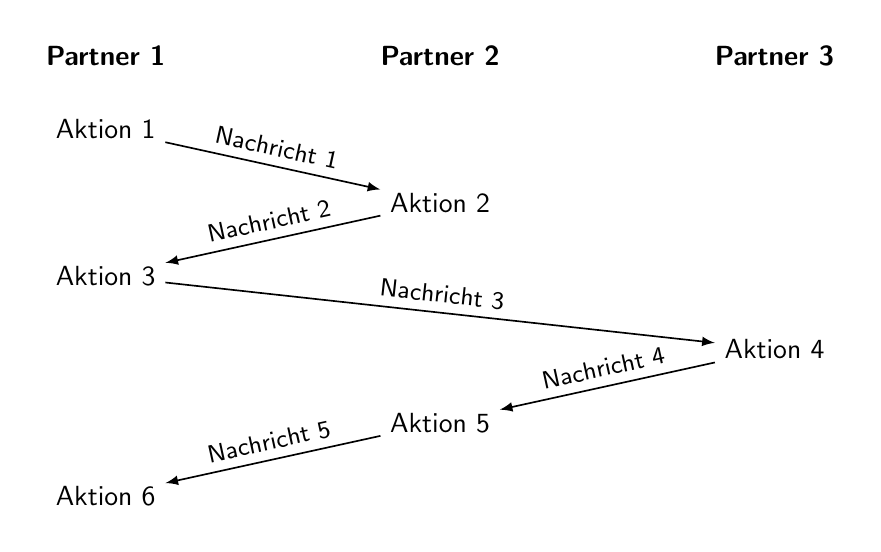
\begin{tikzpicture}[
every node/.append style={font={\sffamily}},
caption/.append style={font={\sffamily\bfseries}},
comm/.style={-latex,semithick},
msg/.style={midway,sloped,above,font={\sffamily\small}},
]
\matrix[row sep=3ex,column sep=25mm] {
\node[caption] {Partner 1};  & \node[caption] {Partner 2}; & \node[caption] {Partner 3}; \\
\node (A1) {Aktion 1}; & & \\
& \node (A2) {Aktion 2}; & \\
\node (A3) {Aktion 3}; & & \\
& & \node (A4) {Aktion 4};\\
& \node (A5) {Aktion 5}; & \\
\node (A6) {Aktion 6}; & & \\
};

\draw[comm] (A1)--(A2) node[msg] {Nachricht 1};
\draw[comm] (A2)--(A3) node[msg] {Nachricht 2};
\draw[comm] (A3)--(A4) node[msg] {Nachricht 3};
\draw[comm] (A4)--(A5) node[msg] {Nachricht 4};
\draw[comm] (A5)--(A6) node[msg] {Nachricht 5};

\end{tikzpicture}%
	}%
	\caption{Netzwerkkommunikationsgraph mit TikZ}%
  \label{fig:net-comm}%
\end{figure}

\begin{figure}[hp]%
	\centering%
	\subfloat[Ursprünglicher Merkmalsraum]{%
		\label{fig:ica-1}%
		\tikzsetnextfilename{ica-1}%
		\resizebox{0.45\textwidth}{!}{%
			\begin{tikzpicture}[
my_plot/.style={draw=none,every mark/.append style={draw=KITblue,fill=KITblue},mark=*,mark size=1.5pt},
]

\begin{axis}[
width=4cm,
height=4cm,
xmin = -1.1,
xmax = 1.1,
xlabel={$m_1$},
ymin = -1.1,
ymax = 1.1,
ylabel={$m_2$},
axis lines=center,
scale only axis,
]

\addplot[my_plot] coordinates {
(0.030,-0.062) (-0.118,-0.004) (0.276,0.236) (0.578,0.566) (-0.143,-0.014)
(0.304,0.257) (0.423,0.535) (0.205,0.344) (0.364,0.365) (-0.327,-0.368)
(0.176,0.310) (-0.298,-0.360) (0.153,0.279) (0.010,0.062) (0.150,0.231)
(-0.301,-0.214) (0.079,0.094) (-0.241,-0.161) (-0.474,-0.461) (0.091,0.173)
(0.541,0.601) (-0.288,-0.153) (0.013,-0.093) (0.290,0.115) (0.194,0.028)
(0.486,0.370) (0.201,0.227) (0.510,0.510) (-0.211,-0.293) (-0.058,0.088)
(0.326,0.176) (-0.591,-0.574) (0.071,0.204) (-0.401,-0.308) (0.206,0.111)
(-0.529,-0.667) (0.064,0.040) (0.032,0.035) (-0.349,-0.291) (0.476,0.316)
(0.625,0.624) (0.312,0.234) (0.076,-0.079) (0.016,0.018) (-0.556,-0.655)
(-0.308,-0.217) (0.248,0.122) (-0.515,-0.428) (-0.121,0.041) (0.260,0.228)
(-0.317,-0.406) (0.650,0.483) (-0.198,-0.097) (-0.427,-0.495) (0.429,0.553)
(-0.432,-0.538) (-0.460,-0.440) (-0.558,-0.654) (0.516,0.586) (-0.230,-0.205)
(0.148,0.199) (-0.417,-0.240) (-0.138,-0.040) (-0.252,-0.403) (0.096,0.010)
(-0.478,-0.339) (0.628,0.650) (0.054,-0.104) (0.502,0.429) (0.051,0.045)
(0.099,0.106) (0.344,0.214) (-0.359,-0.334) (0.291,0.187) (0.176,0.217)
(0.329,0.362) (-0.270,-0.116) (-0.136,-0.008) (-0.446,-0.533) (0.653,0.585)
(0.474,0.540) (0.093,0.136) (0.356,0.473) (0.232,0.217) (0.592,0.659)
(-0.326,-0.170) (-0.683,-0.497) (-0.484,-0.357) (-0.607,-0.635) (-0.044,-0.041)
(-0.681,-0.533) (-0.306,-0.401) (0.189,0.334) (0.420,0.259) (0.040,0.086)
(-0.148,-0.303) (-0.585,-0.507) (0.424,0.330) (0.597,0.688) (0.211,0.271)
(-0.429,-0.360) (0.280,0.188) (0.375,0.252) (-0.505,-0.528) (-0.064,-0.043)
(-0.257,-0.140) (0.302,0.262) (-0.228,-0.293) (0.154,0.122) (-0.549,-0.403)
(0.034,-0.027) (0.207,0.122) (-0.538,-0.648) (-0.601,-0.664) (-0.623,-0.433)
(-0.552,-0.417) (-0.094,-0.166) (0.469,0.496) (0.580,0.497) (0.212,0.159)
(0.515,0.627) (-0.070,-0.167) (-0.101,-0.015) (-0.244,-0.328) (-0.372,-0.477)
(0.256,0.199) (-0.607,-0.560) (-0.462,-0.554) (0.132,0.086) (0.066,0.050)
(0.230,0.157) (-0.502,-0.556) (0.666,0.490) (0.407,0.425) (-0.219,-0.355)
(-0.250,-0.285) (0.266,0.159) (-0.263,-0.412) (0.028,0.091) (-0.086,0.043)
(-0.633,-0.504) (-0.420,-0.399) (0.378,0.380) (-0.008,-0.163) (-0.226,-0.278)
(0.148,0.193) (-0.629,-0.582) (0.586,0.450) (0.025,0.136) (-0.445,-0.360)
};

\end{axis}
\end{tikzpicture}
		}%
	}%
	\hfill%
	\subfloat[Transienter Merkmalsraum (Nach Whitening, z.\,B. durch \gls{ac:PCA} inkl. Normalisierung)]{%
		\label{fig:ica-2}%
		\tikzsetnextfilename{ica-2}%
		\resizebox{0.45\textwidth}{!}{%
			\begin{tikzpicture}[
my_plot/.style={draw=none,every mark/.append style={draw=KITblue,fill=KITblue},mark=*,mark size=1.5pt},
]

\begin{axis}[
width=4cm,
height=4cm,
xmin = -1.1,
xmax = 1.1,
xlabel={$m'_1$},
ymin = -1.1,
ymax = 1.1,
ylabel={$m'_2$},
axis lines=center,
scale only axis,
]

\addplot[my_plot] coordinates {
(-0.273,-0.278) (0.267,0.398) (0.117,-0.289) (0.483,-0.399) (0.293,0.455)
(0.120,-0.326) (0.747,0.049) (0.640,0.265) (0.329,-0.231) (-0.430,0.090)
(0.597,0.269) (-0.471,0.014) (0.549,0.259) (0.180,0.141) (0.401,0.136)
(0.014,0.439) (0.120,-0.008) (0.044,0.379) (-0.384,0.338) (0.349,0.173)
(0.681,-0.175) (0.183,0.566) (-0.335,-0.309) (-0.310,-0.678) (-0.368,-0.593)
(0.057,-0.637) (0.266,-0.054) (0.457,-0.325) (-0.457,-0.098) (0.425,0.450)
(-0.196,-0.631) (-0.474,0.426) (0.500,0.334) (-0.059,0.516) (-0.127,-0.402)
(-0.926,-0.054) (-0.019,-0.107) (0.038,-0.012) (-0.122,0.388) (-0.094,-0.754)
(0.560,-0.398) (0.026,-0.418) (-0.439,-0.488) (0.021,-0.004) (-0.822,0.075)
(0.020,0.454) (-0.190,-0.516) (-0.180,0.573) (0.420,0.535) (0.130,-0.255)
(-0.575,-0.050) (0.039,-0.885) (0.151,0.410) (-0.607,0.078) (0.790,0.077)
(-0.736,-0.026) (-0.348,0.349) (-0.817,0.082) (0.692,-0.130) (-0.126,0.216)
(0.301,0.052) (0.202,0.765) (0.195,0.363) (-0.719,-0.267) (-0.195,-0.306)
(0.024,0.696) (0.635,-0.338) (-0.469,-0.483) (0.215,-0.523) (0.028,-0.048)
(0.113,-0.042) (-0.116,-0.587) (-0.242,0.298) (-0.078,-0.479) (0.291,0.003)
(0.405,-0.114) (0.259,0.605) (0.297,0.450) (-0.684,0.038) (0.365,-0.607)
(0.644,-0.112) (0.223,0.062) (0.701,0.104) (0.158,-0.192) (0.752,-0.185)
(0.214,0.646) (-0.007,0.960) (-0.020,0.667) (-0.635,0.308) (-0.029,0.037)
(-0.131,0.849) (-0.587,-0.076) (0.645,0.292) (-0.150,-0.724) (0.184,0.102)
(-0.638,-0.344) (-0.270,0.594) (0.073,-0.536) (0.833,-0.122) (0.385,0.036)
(-0.160,0.468) (-0.048,-0.437) (-0.065,-0.586) (-0.531,0.254) (0.010,0.099)
(0.151,0.495) (0.141,-0.305) (-0.417,-0.039) (0.033,-0.188) (-0.016,0.763)
(-0.166,-0.191) (-0.093,-0.373) (-0.843,0.031) (-0.746,0.204) (0.060,0.933)
(-0.055,0.733) (-0.320,-0.144) (0.510,-0.221) (0.252,-0.601) (0.018,-0.283)
(0.829,-0.011) (-0.381,-0.230) (0.190,0.308) (-0.492,-0.081) (-0.679,-0.062)
(0.042,-0.326) (-0.391,0.520) (-0.717,0.032) (-0.032,-0.214) (0.009,-0.085)
(-0.034,-0.355) (-0.627,0.168) (0.022,-0.923) (0.424,-0.209) (-0.641,-0.245)
(-0.339,0.060) (-0.110,-0.472) (-0.722,-0.253) (0.230,0.160) (0.345,0.421)
(-0.147,0.768) (-0.309,0.326) (0.348,-0.233) (-0.513,-0.434) (-0.372,-0.002)
(0.278,0.031) (-0.413,0.531) (0.082,-0.757) (0.384,0.297) (-0.122,0.523)
};

\end{axis}
\end{tikzpicture}%
		}%
	}%
	\hfill%
	\subfloat[Transformierter Merkmalsraum]{%
		\label{fig:ica-3}%
		\tikzsetnextfilename{ica-3}%
		\resizebox{0.45\textwidth}{!}{%
			\begin{tikzpicture}[
my_plot/.style={draw=none,every mark/.append style={draw=KITblue,fill=KITblue},mark=*,mark size=1.5pt},
]

\begin{axis}[
width=4cm,
height=4cm,
xmin = -1.1,
xmax = 1.1,
xlabel={$m''_1$},
ymin = -1.1,
ymax = 1.1,
ylabel={$m''_2$},
axis lines=center,
scale only axis,
]

\addplot[my_plot] coordinates {
(-0.389,-0.004) (0.470,0.093) (-0.122,-0.287) (0.059,-0.623) (0.529,0.115)
(-0.146,-0.316) (0.563,-0.493) (0.640,-0.265) (0.069,-0.396) (-0.241,0.367)
(0.613,-0.232) (-0.323,0.342) (0.572,-0.205) (0.227,-0.027) (0.379,-0.188)
(0.320,0.300) (0.079,-0.090) (0.299,0.237) (-0.033,0.510) (0.369,-0.124)
(0.358,-0.605) (0.530,0.271) (-0.455,0.019) (-0.699,-0.260) (-0.680,-0.159)
(-0.410,-0.491) (0.150,-0.226) (0.093,-0.554) (-0.393,0.254) (0.619,0.017)
(-0.584,-0.307) (-0.034,0.636) (0.590,-0.118) (0.323,0.406) (-0.374,-0.194)
(-0.693,0.617) (-0.089,-0.062) (0.018,-0.035) (0.188,0.361) (-0.600,-0.467)
(0.114,-0.678) (-0.277,-0.314) (-0.655,-0.035) (0.012,-0.018) (-0.528,0.634)
(0.335,0.306) (-0.499,-0.230) (0.278,0.532) (0.676,0.081) (-0.088,-0.272)
(-0.442,0.371) (-0.599,-0.654) (0.397,0.183) (-0.374,0.484) (0.613,-0.504)
(-0.539,0.502) (0.001,0.493) (-0.520,0.635) (0.398,-0.581) (0.063,0.242)
(0.249,-0.176) (0.684,0.398) (0.395,0.119) (-0.697,0.320) (-0.354,-0.078)
(0.509,0.475) (0.210,-0.688) (-0.674,-0.010) (-0.218,-0.522) (-0.014,-0.053)
(0.050,-0.110) (-0.498,-0.333) (0.040,0.382) (-0.394,-0.284) (0.208,-0.204)
(0.206,-0.367) (0.611,0.245) (0.528,0.108) (-0.457,0.510) (-0.171,-0.688)
(0.376,-0.535) (0.202,-0.114) (0.569,-0.422) (-0.024,-0.247) (0.401,-0.663)
(0.608,0.305) (0.674,0.684) (0.457,0.486) (-0.231,0.667) (0.005,0.047)
(0.508,0.693) (-0.469,0.362) (0.663,-0.250) (-0.618,-0.406) (0.203,-0.058)
(-0.694,0.208) (0.229,0.611) (-0.327,-0.431) (0.503,-0.676) (0.298,-0.247)
(0.217,0.444) (-0.343,-0.275) (-0.460,-0.368) (-0.196,0.555) (0.077,0.063)
(0.457,0.243) (-0.116,-0.315) (-0.322,0.267) (-0.110,-0.157) (0.528,0.550)
(-0.253,-0.018) (-0.329,-0.198) (-0.574,0.618) (-0.384,0.672) (0.702,0.617)
(0.480,0.557) (-0.329,0.124) (0.205,-0.517) (-0.247,-0.604) (-0.188,-0.213)
(0.578,-0.594) (-0.432,0.106) (0.352,0.083) (-0.406,0.291) (-0.523,0.436)
(-0.201,-0.260) (0.091,0.644) (-0.484,0.530) (-0.173,-0.129) (-0.054,-0.067)
(-0.275,-0.227) (-0.325,0.562) (-0.637,-0.668) (0.152,-0.447) (-0.626,0.280)
(-0.197,0.283) (-0.411,-0.256) (-0.690,0.332) (0.276,-0.050) (0.542,0.054)
(0.439,0.647) (0.012,0.449) (0.081,-0.411) (-0.670,0.056) (-0.265,0.262)
(0.218,-0.175) (0.083,0.668) (-0.477,-0.594) (0.482,-0.061) (0.284,0.456)
};

\end{axis}
\end{tikzpicture}%
		}%
}%
\caption{Diagramme mit TikZ direkt in LaTeX (hier: Die Schritte der \enquote{Independent component analysis})}%
\label{fig:ica}%
\end{figure}

\begin{figure}[hp]
	\centering%
	\subfloat[Ungünstige Projektion]{%
		\label{fig:pca-1}%
		\tikzsetnextfilename{pca-1}%
		\resizebox{0.48\textwidth}{!}{%
			\begin{tikzpicture}[
my_plot_1/.style={draw=none,every mark/.append style={draw=KITblue,fill=KITblue},mark=*},
my_plot_2/.style={draw=none,every mark/.append style={draw=KITred,fill=KITred},mark=*},
trans_arrow/.style={semithick,KITorange,-latex},
]

\begin{axis}[
width=4cm,
height=4cm,
xmin = -0.2,
xmax = 2.3,
xlabel={$m_1$},
ymin = -0.2,
ymax = 2.3,
ylabel={$m_2$},
xticklabel=\empty,
yticklabel=\empty,
axis lines=center,
clip=false,
scale only axis,
]

\addplot[my_plot_1] coordinates {
(1.3,0.38)
(1.42,0.71)
(1.48,0.60)
(1.64,0.54)
(1.65,0.81)
(1.68,0.89)
(1.79,1.11)
(1.88,1.18)
(1.89,1.46)
(1.94,1.35)
(1.86,1.65)
(2.02,1.83)
(2.12,1.83)
(2.19,2.26)
(2.21,2.07)
};

\addplot[my_plot_2] coordinates {
(1.28,0.58)
(1.33,0.93)
(1.54,1.03)
(1.54,1.26)
(1.51,1.41)
(1.72,1.52)
(1.76,1.87)
(1.80,1.90)
(1.90,2.00)
(1.91,2.27)
(2.05,2.40)
};

\coordinate(CoM) at (axis cs:1.71,1.38) {};

\draw[trans_arrow] (axis cs:0,0)--(CoM) node[midway,above left] {$m_0$};

\end{axis}

\begin{axis}[
width=5cm,
height=2.5cm,
xmin = -1.5,
xmax = 1.5,
xlabel={$m'_1$},
ymin = -0.75,
ymax = 0.75,
ylabel={$m'_2$},
axis lines=center,
xlabel style={anchor=north west},
ylabel style={anchor=south west},
xticklabel=\empty,
yticklabel=\empty,
clip=false,
anchor=origin,
at={(CoM)},
rotate around={65:(current axis.origin)},
clip=false,
scale only axis
]

\addplot+[my_plot_1] coordinates {
(-2,-0.0510)
(-2,-0.0203)
(-2,-0.1212)
(-2,-0.2916)
(-2,-0.1865)
(-2,-0.1799)
(-2,-0.1866)
(-2,-0.2386)
(-2,-0.1293)
(-2,-0.2211)
(-2,-0.0218)
(-2,-0.0908)
(-2,-0.1814)
(-2,-0.0631)
(-2,-0.1615)
};

\addplot+[my_plot_2] coordinates {
(-2,0.0516)
(-2,0.1542)
(-2,0.0062)
(-2,0.1034)
(-2,0.1939)
(-2,0.0501)
(-2,0.1618)
(-2,0.1382)
(-2,0.0898)
(-2,0.1949)
(-2,0.1229)
};

\draw[trans_arrow,shorten <=2pt,shorten >=3pt] (axis cs:-1.5,0)--(axis cs:-2,0) node[midway,right,font={\footnotesize},align=left] {Projektion\\auf $e_2$};
\draw[semithick] (axis cs:-2,-0.5)--(axis cs:-2,0.4);

\addplot+[my_plot_1] coordinates {
(-1.0796,-1.5)
(-0.7298,-1.5)
(-0.8041,-1.5)
(-0.7909,-1.5)
(-0.5420,-1.5)
(-0.4568,-1.5)
(-0.2109,-1.5)
(-0.1094,-1.5)
(0.1486,-1.5)
(0.0700,-1.5)
(0.3081,-1.5)
(0.5389,-1.5)
(0.5811,-1.5)
(1.0004,-1.5)
(0.8367,-1.5)
};

\addplot+[my_plot_2] coordinates {
(-0.9068,-1.5)
(-0.5684,-1.5)
(-0.3891,-1.5)
(-0.1806,-1.5)
(-0.0573,-1.5)
(0.1311,-1.5)
(0.4652,-1.5)
(0.5093,-1.5)
(0.6422,-1.5)
(0.8911,-1.5)
(1.0681,-1.5)
};

\draw[trans_arrow,shorten <=2pt,shorten >=3pt] (axis cs:0,-0.75)--(axis cs:0,-1.5) node[midway,anchor=north east,font={\footnotesize},align=left] {Projektion\\auf $e_1$};
\draw[semithick] (axis cs:-1.3,-1.5)--(axis cs:1.3,-1.5);

\end{axis}

\end{tikzpicture}%
		}%
	}\hfill%
	\subfloat[Zielführende Projektion]{%
		\label{fig:pca-2}%
		\tikzsetnextfilename{pca-2}%
		\resizebox{0.48\textwidth}{!}{%
			\begin{tikzpicture}[
my_plot_1/.style={draw=none,every mark/.append style={draw=KITblue,fill=KITblue},mark=*},
my_plot_2/.style={draw=none,every mark/.append style={draw=KITred,fill=KITred},mark=*},
trans_arrow/.style={semithick,KITorange,-latex},
]

\begin{axis}[
width=4cm,
height=4cm,
xmin = -0.2,
xmax = 2.3,
xlabel={$m_1$},
ymin = -0.2,
ymax = 2.3,
ylabel={$m_2$},
xticklabel=\empty,
yticklabel=\empty,
axis lines=center,
clip=false,
scale only axis,
]

\addplot[my_plot_1] coordinates {
(1.3,0.38)
(1.28,0.58)
(1.42,0.71)
(1.48,0.60)
(1.64,0.54)
(1.33,0.93)
(1.65,0.81)
(1.68,0.89)
(1.54,1.03)
(1.54,1.26)
(1.79,1.11)
(1.88,1.18)
(1.51,1.41)
};

\addplot[my_plot_2] coordinates {
(1.72,1.52)
(1.89,1.46)
(1.94,1.35)
(1.86,1.65)
(1.76,1.87)
(1.80,1.90)
(1.90,2.00)
(2.02,1.83)
(2.12,1.83)
(1.91,2.27)
(2.19,2.26)
(2.21,2.07)
(2.05,2.40)
};

\coordinate(CoM) at (axis cs:1.71,1.38) {};

\draw[trans_arrow] (axis cs:0,0)--(CoM) node[midway,above left] {$m_0$};

\end{axis}

\begin{axis}[
width=5cm,
height=2.5cm,
xmin = -1.5,
xmax = 1.5,
xlabel={$m'_1$},
ymin = -0.75,
ymax = 0.75,
ylabel={$m'_2$},
axis lines=center,
xlabel style={anchor=north west},
ylabel style={anchor=south west},
xticklabel=\empty,
yticklabel=\empty,
clip=false,
anchor=origin,
at={(CoM)},
rotate around={65:(current axis.origin)},
clip=false,
scale only axis
]

\addplot+[my_plot_1] coordinates {
(-2,-0.0510)
(-2,0.0516)
(-2,-0.0203)
(-2,-0.1212)
(-2,-0.2916)
(-2,0.1542)
(-2,-0.1865)
(-2,-0.1799)
(-2,0.0062)
(-2,0.1034)
(-2,-0.1866)
(-2,-0.2386)
(-2,0.1939)
};

\addplot+[my_plot_2] coordinates {
(-2,0.0501)
(-2,-0.1293)
(-2,-0.2211)
(-2,-0.0218)
(-2,0.1618)
(-2,0.1382)
(-2,0.0898)
(-2,-0.0908)
(-2,-0.1814)
(-2,0.1949)
(-2,-0.0631)
(-2,-0.1615)
(-2,0.1229)
};

\draw[trans_arrow,shorten <=2pt,shorten >=3pt] (axis cs:-1.5,0)--(axis cs:-2,0) node[midway,right,font={\footnotesize},align=left] {Projektion\\auf $e_2$};
\draw[semithick] (axis cs:-2,-0.5)--(axis cs:-2,0.4);

\addplot+[my_plot_1] coordinates {
(-1.0796,-1.5)
(-0.9068,-1.5)
(-0.7298,-1.5)
(-0.8041,-1.5)
(-0.7909,-1.5)
(-0.5684,-1.5)
(-0.5420,-1.5)
(-0.4568,-1.5)
(-0.3891,-1.5)
(-0.1806,-1.5)
(-0.2109,-1.5)
(-0.1094,-1.5)
(-0.0573,-1.5)
};

\addplot+[my_plot_2] coordinates {
(0.1311,-1.5)
(0.1486,-1.5)
(0.0700,-1.5)
(0.3081,-1.5)
(0.4652,-1.5)
(0.5093,-1.5)
(0.6422,-1.5)
(0.5389,-1.5)
(0.5811,-1.5)
(0.8911,-1.5)
(1.0004,-1.5)
(0.8367,-1.5)
(1.0681,-1.5)
};

\draw[trans_arrow,shorten <=2pt,shorten >=3pt] (axis cs:0,-0.75)--(axis cs:0,-1.5) node[midway,anchor=north east,font={\footnotesize},align=left] {Projektion\\auf $e_1$};
\draw[semithick] (axis cs:-1.3,-1.5)--(axis cs:1.3,-1.5);

\end{axis}

\end{tikzpicture}%
		}%
	}%
	\caption{Aufwändiges Diagramm mit TikZ (hier: Probleme der \enquote{Principal component analysis})}%
	\label{fig:pca}%
\end{figure}
%%%%%%%%%%%%%%%%%%%%%%%%%%%%%%%%%%%%%%%%%%%%%%%%%%%%%%%%%%%%
\section{Tabellen}%
\label{sec:Tabellen}
%%%%%%%%%%%%%%%%%%%%%%%%%%%%%%%%%%%%%%%%%%%%%%%%%%%%%%%%%%%%
Für eine ausführliche Erläuterung auch über gute und schlechte Tabellen
und deren Gestaltung empfiehlt sich die Lektüre des entsprechenden Artikels im \LaTeX{}"=Kompendium auf Wikibooks%
\footnote{\url{https://de.wikibooks.org/wiki/LaTeX-Kompendium:_Tabellen}}
sowie die Dokumentation des \pkg{booktabs}-Pakets \cite{Fear2005}.
\Ua stellt dieses Paket die Befehle
\begin{itemize*}
	\item \lstinline|\toprule|
	\item \lstinline|\midrule|
	\item \lstinline|\bottomrule|
\end{itemize*}
zur Verfügung.

Eine einfache Tabelle hat den folgenden Code:

\begin{latex}[caption={Einfache Tabelle in \LaTeX},label={lst:tabellenbeispiel}]
\begin{table}%
	\centering%
	\begin{tabularx}{\columnwidth}{l l X}%
		\toprule%
		Datei       &  Bedeutung    &  Benutzerinteraktion \\%
		\midrule%
		Diss.tex  &  Hauptdatei   &  nein     \\%
		images/   &  Bilder       &  ja       \\%
		content/  &  Kapitel      &  ja       \\%
		\bottomrule%
	\end{tabularx}%
	\caption{Dateien der Vorlage}%
	\label{tab:tabellenbeispiel}%
\end{table}
\end{latex}

Das Ergebnis sieht man in \cref{tab:tabellenbeispiel}.

\begin{table}%
	\centering%
	\begin{tabular}{l l l}%
		\toprule%
		Datei       &  Bedeutung    &  Benutzerinteraktion \\%
		\midrule%
		Diss.tex  &  Hauptdatei   &  nein     \\%
		images/   &  Bilder       &  ja       \\%
		content/  &  Kapitel      &  ja       \\%
		\bottomrule%
	\end{tabular}%
	\caption{Dateien der Vorlage}%
	\label{tab:tabellenbeispiel}%
\end{table}

Etwas komplizierter wird es, wenn man eine Tabelle mit alternierender Farbe einfügen möchte (\cref{tab:AlternierendeZeilenfarben}).

\begin{table}
\caption{Tabelle mit alternierender Zeilenfarbe}%
\label{tab:AlternierendeZeilenfarben}%
	\tablestyle%
	\tablealtcolored%
	\begin{tabular}{*{2}{v{0.45\textwidth}}}
		\toprule%
		\tableheadcolor%
		\tableheadformat Tabellenkopf &	\tableheadformat Tabellenkopf
		\tabularnewline%
		\midrule%
		%% Zwischenkopf ---------------------------------------------
		\multicolumn{2}{>{\columncolor{tablesubheadcolor}}l}{\bfseries\color{KITblue} Zwischenkopf}%
		\tabularnewline%
		%%-----------------------------------------------------------
		Inhalt  & Inhalt \tabularnewline
		Inhalt  & Inhalt \tabularnewline
		Inhalt  & Inhalt \tabularnewline
		%% Zwischenkopf ---------------------------------------------
		\multicolumn{2}{>{\columncolor{tablesubheadcolor}}l}{\bfseries\color{KITgreen} Zwischenkopf}%
		\tabularnewline
		%%-----------------------------------------------------------
		Inhalt  & Inhalt \tabularnewline
		Inhalt  & Inhalt \tabularnewline
		\bottomrule%
	\end{tabular}%
\end{table}

%% ------------------------------------------------------------
Lange Tabellen, die umbrochen werden sollen, können mit
\lstinline|\LTXtable{\textwidth}{Datei}|
eingebunden werden, wobei die Tabelle in eine Datei ausgelagert werden muss.
Ein Beispiel dafür sieht man in \cref{tab:MehrseitigeTabelle}.

\IfDefined{LTXtable}{%
	%--Einstellungen für Tabellen ----------
	\colorlet{tablerowcolor}{gray!10.0}%
	\renewcommand\tableheadcolor{\rowcolor{tableheadcolor}}%
	\renewcommand\tablehead{%
			\tableheadfontsize%
			\sffamily\bfseries%
			\slshape%
			\color{black}%
	}%
	%---------------------------------------
	{
		\tablestyle%
		%\tablealtcolored
		\rowcolors{1}{tablerowcolor}{white!100}%
		 \LTXtable{\textwidth}{tables/LongTableExample.tex}%
	}%
} % End If 
%
%
%
Sollten eine Tabelle einmal so breit sein, dass sie nicht mehr horizontal auf
eine Seite passt, so ist es natürlich möglich, diese mithilfe des Pakets
\printkeyword{rotfloat} \parencite{Sommerfeldt2004} in eine
\printkeyword{sidewaystable} statt in eine \printkeyword{table}-Umgebung zu setzen.
Also so:
\begin{latex}[caption={Gedrehte Tabelle},label={lst:rotated-table}]
\begin{sidewaystable}
  \centering%
  \begin{tabular}{...}%
    ...
  \end{tabular}%
  \caption{Bezeichnung}%
  \label{Referenzmarke}%
\end{sidewaystable}%
\end{latex}

Das Ergebnis sieht man in \cref{tab:ex-sideways}.

%% Um 90° gedrehte Tabelle
%
\begin{sidewaystable}[p]
\scriptsize%
%\tiny
\centering%
\begin{tabular}{l M M M M M}%
\toprule%
\addlinespace[0pt]%
 & \multicolumn{5}{c}{\bfseries Level} \tabularnewline
 & \multicolumn{2}{c}{\bfseries Qualitative} & \multicolumn{3}{c}{\bfseries Quantitative} \tabularnewline
 & \bfseries\centering Nominal & \bfseries\centering Ordinal & \bfseries\centering Interval & \bfseries\centering Ratio & \bfseries\centering Absolute \tabularnewline \addlinespace[0pt]\midrule\addlinespace[0pt]
Empirical relation &
\begin{tabitemize}\item[$\sim$] Equivalence\end{tabitemize} &
\begin{tabitemize}\item[$\sim$] Equivalence\item[$\prec$] Ordering\end{tabitemize} &
\begin{tabitemize}\item[$\sim$] Equivalence\item[$\prec$] Ordering\end{tabitemize} &
\begin{tabitemize}\item[$\sim$] Equivalence\item[$\prec$] Ordering\strut\end{tabitemize} &
\begin{tabitemize}\item[$\sim$] Equivalence\item[$\prec$] Ordering\strut\end{tabitemize} \tabularnewline \midrule
Empirical operation &
 &
 &
\begin{tabitemize}\item[$\oplus$] Addition\end{tabitemize} &
\begin{tabitemize}\item[$\oplus$] Addition\item[$\otimes$] Multiplication\strut\end{tabitemize} &
\begin{tabitemize}\item[$\oplus$] Addition\item[$\otimes$] Multiplication\strut\end{tabitemize} \tabularnewline \midrule
Feasable transformation &
$m' = f( m )$ for $f$ bij.\strut &
$m' = f( m )$ for $f$ mon.\strut &
$m' = am + b$ for $a>0$\strut &
$m' = am$ for $a>0$\strut &
$m' = m$\strut \tabularnewline \midrule
Examples of features &
\begin{tabitemize}\item Telephone numbers\item Postal codes\item Gender\strut\end{tabitemize} &
\begin{tabitemize}\item Grades\item Degree of hardness\item Wind intensity\strut\end{tabitemize} &
\begin{tabitemize}\item Temperatur in F\textdegree\item Calendric time\item Geographic altitude\strut\end{tabitemize} &
\begin{tabitemize}\item Temperatur in K\item Mass\item Length\item Electric current\strut\end{tabitemize} &
\begin{tabitemize}\item Quantum numbers\item Error number\strut\end{tabitemize} \tabularnewline \midrule
Range of features &
\begin{tabitemize}\item Numbers\item Names\item Symbols\strut\end{tabitemize} &
Natural numbers &
Real numbers &
Real, positive numbers &
Natural numbers \tabularnewline \midrule
Expressiveness & low & \dots & \dots & \dots & high\strut \tabularnewline \addlinespace[0pt]
\bottomrule%
\end{tabular}%
\caption{Beispiel für eine breite, gedrehte Tabelle (hier: Taxonomie der Maßskalen)}%
\label{tab:ex-sideways}%
\end{sidewaystable}
%%%%%%%%%%%%%%%%%%%%%%%%%%%%%%%%%%%%%%%%%%%%%%%%%%%%%%%%%%%%
\section{Mathematische Sätze, Lemmas, Definitionen etc.}%
\label{sec:Theoreme}
%%%%%%%%%%%%%%%%%%%%%%%%%%%%%%%%%%%%%%%%%%%%%%%%%%%%%%%%%%%%
%
Für eine mathematische Ausarbeitung gibt es LaTeX-\glspl{gls:umgebung}, um
\index{Satz|see{Theorem}}\index{Theorem}Sätze (Theoreme), \index{Lemma|see{Theorem}}Lemma,
\index{Beispiel|see{Theorem}}Beispiele etc. im üblichen Stil von
Mathematik-Büchern zu setzen und zu referenzieren. Vordefiniert sind die
\glspl{gls:umgebung}
\begin{itemize*}
  \item \texttt{theorem} für Sätze
  \item \texttt{definition} für Definitionen
  \item \texttt{lemma} für Lemma
  \item \texttt{corollary} für Korollare
  \item \texttt{proposition} für Propositionen
\end{itemize*}
Die übliche Verwendung ist
\begin{latex}[caption={Beispiel für Theorem-Umgebungen},label={lst:ntheorem}]
\begin{theorem}[Optionaler Name]\label{thm:my-theorem}
...
\end{theorem}
\end{latex}
Weitere Informationen findet man in der Dokumentation zum \texttt{ntheorem}-Paket
\parencite{May2011}. Das Ganze sieht dann beispielsweise wie folgt aus.

\begin{theorem}[Theorem von Arthur Dent]
\label{thm:arthur-dent} Die Antwort auf die Frage nach dem Leben, dem Universum und den ganzen Rest ist 42.
\end{theorem}

\begin{definition}
\LaTeX{} ist eine von Leslie Lamport 1980 entwickelter Satz von Makros zur Erweiterung von \TeX.
\end{definition}

\begin{proposition}[Zweifelhafte Folgerung]
LaTeX ist schön. Beweis folgt unmittelbar aus \cref{thm:arthur-dent}.
\end{proposition}

%%%%%%%%%%%%%%%%%%%%%%%%%%%%%%%%%%%%%%%%%%%%%%%%%%%%%%%%%%%%
\section{Quellcode-Listings}%
\index{Listing!Gestaltungsstil}%
\label{sec:Listings}
%%%%%%%%%%%%%%%%%%%%%%%%%%%%%%%%%%%%%%%%%%%%%%%%%%%%%%%%%%%%
%
Zum Einbinden und formatieren von \index{Code|see{Listing}}Quellcode"=Beispielen
-- sog. \index{Listing}Listings -- wird das Paket \pkg{listings}
\parencite{Hoffmann2014} verwendet.
Das Hervorheben von \index{Schlusselwort@Schlüsselwort}Schlüsselwörtern
wird von LaTeX automatisch erledigt,
wenn die korrekte Sprache des Listings angegeben ist.
Dies geschieht mit Hilfe der Option \printkeyword{language}
oder durch die Angabe eines entsprechend definierten Gestaltungsstils.

Im Befehl \lstinline|\lstset{...}|,
welcher in der Datei \printfilepath{preambel/preambel.tex} zu finden ist,
kann man einen globalen Stil für alle Listings vorgeben
(welcher jedoch bei Bedarf im Einzelfall überrufen werden kann).
Aktuell ist der etwas weiter oben im Code mit dem Befehl
\lstinline|\lstdefinestyle{...}| vordefinierte Stil
\printkeyword{latex} als Standardgestaltungsstil ausgewählt.

Neben \printkeyword{latex} sind in der Datei \printfilepath{preambel/preambel.tex}
auch noch \printkeyword{java} und \printkeyword{C++} als Gestaltungsstile vordefiniert.
Bei Bedarf lassen sich dort weitere Stile definieren und auswählen.

Zur Vereinfachung der Einbindung wurden zusätzlich Umgebungen
\printkeyword{latex}, \printkeyword{java} und \printkeyword{C++}
vordefiniert, die im Code mit \lstinline|\begin{<name>}...\end{<name>}|
direkt verwendet werden können (s. \cref{lst:java-listing}).
%
So bewirkt beispielsweise
%
\begin{latex}[caption={Beispiel eines Listings in Java},label={lst:java-listing}]
\begin{java}[caption={A Java Hello-World example},%
             label={lst:hello-world}]
public class HelloWorld {
  public static void main( String[] args ) {
    System.out.println( "HelloWorld" );
  }
}
\end{java}
\end{latex}
%
das folgende Ergebnis:
%
\begin{C++}[caption={A Java Hello-World example},label={lst:hello-world}]
public class HelloWorld {
  public static void main( String[] args ) {
    System.out.println( "HelloWorld" );
  }
}
\end{C++}

Man beachte, dass anders als bei Abbildungen und Tabellen
die Bezeichnung (\texttt{caption}) und die Referenzmarke (\texttt{label})
nicht als gesonderte Befehle sondern als optionale Argumente übergeben werden.
Dies liegt daran, dass ein Listing in der Regel keine Fließumgebung ist,
sondern an der Stelle im Text erscheint, an der sie im Code auch steht.
Ferner folgt ein Listing den ganz normalen Seitenumbruchsregeln.
Das heißt, überlanger Code wird einfach umgebrochen. 
Um ein Listing zu einem Fließobjekt zu machen, muss das optionale Argument
\texttt{float=<tbp>} angegeben werden.
Die \index{Platzierung}Plazierungsangabe \enquote{\texttt{h}} für \enquote{hier}
ist nicht erlaubt. Denn dies ist das Standardverhalten ohne \texttt{float}.
%%%%%%%%%%%%%%%%%%%%%%%%%%%%%%%%%%%%%%%%%%%%%%%%%%%%%%%%%%%%
\section{Querverweise und Hyperlinks}%
\label{sec:Querverweise}
%%%%%%%%%%%%%%%%%%%%%%%%%%%%%%%%%%%%%%%%%%%%%%%%%%%%%%%%%%%%
%
Querverweise sollten nicht mit dem Befehl \lstinline|\ref{...}| gesetzt werden,
sondern mit \lstinline|\cref{...}| und verwandten Befehlen aus dem Paket
\pkg{cleveref} \cite{Cubitt2013}.
Diese Befehle haben den Vorteil nicht nur die Nummer zu referenzieren,
sondern auch den Typ mit anzugeben.
Hinzu kommt eine intelligente Verwendung der Pluralform und
\index{Sortierung}Sortierung bei Mehrfachaufzählungen auch unterschiedlichen Typs.
Will man \bspw auf zwei Abbildungen und eine Tabelle mit den Marken (\enquote{Labels})
%
\begin{itemize*}
\item \texttt{fig:subfloat-example}
\item \texttt{tab:files-dirs-of-template}
\item \texttt{fig:kit-colors}
\end{itemize*}
%
verweisen, so schreibt man einfach per Komma getrennt
%
\begin{latex}[caption={Cleveres Referenzieren mit \bs cref},label={lst:cref}]
\cref{fig:subfloat-example,
      tab:ex-sideways,
      fig:kit-colors}
\end{latex}
%
und erhält als Resultat
\enquote{\cref{fig:subfloat-example,tab:ex-sideways,fig:kit-colors}}.

\index{URL}\index{Internetadresse|see{URL}}Internetadressen werden in das Kommando \lstinline|\url{...}| eingefasst.
Außerdem besteht die Möglichkeit mit dem Befehl \lstinline|\href{<URL>}{Text}| eine Textstelle mit einem Hyperlink zu versehen.
%%%%%%%%%%%%%%%%%%%%%%%%%%%%%%%%%%%%%%%%%%%%%%%%%%%%%%%%%%%%
\section{Mathematik}%
\label{sec:Mathe}
%%%%%%%%%%%%%%%%%%%%%%%%%%%%%%%%%%%%%%%%%%%%%%%%%%%%%%%%%%%%
%
Grundsätzlich gilt, was in \parencites{ams1999a}{ams1999b} steht. In der Datei
\printfilepath{preambel/05-math.tex} sind eine Menge Kurzkommandos definiert, um eine
einheitliche Typografie von \index{Skalare}Skalaren, \index{Vektoren}Vektoren,
\index{Matrizen}Matrizen, \index{Zufallsvariablen}Zufallsvariablen etc.
zur vereinfachen. In diese Dateien einfach mal reinschauen, welche Kurzkommandos
es gibt.

Auf zwei besondere Kommandos wird näher eingegangen, weil dies häufig falsch
gemacht wird.
\begin{itemize}
  \item Für die Matrixtransponierte gibt es das Kommando \verb#\Tr#, also
	\verb#$A^{\Tr}$# liefert $A^{\Tr}$
	
	\item Bei \index{Integral}Integralen muss das \enquote{Differential-d} gemäß
	ISO in aufrechter Schrift als Operator gesetzt sein mit einem kleinen Abstand
	zum Integranden. Hierfür gibt es das spezielle Kommando \verb#\diff#. Also
	\begin{equation}
	 \int^1_0 x^2 d x = \frac{1}{3} \qquad \text{(falsche Typografie!)}
	\end{equation}
	ist falsch, während \verb#\int^1_0 x^2 \diff x = \frac{1}{3}# das Richtige
	liefert
	\begin{equation}
	 \int^1_0 x^2 \diff x = \frac{1}{3} \qquad \text{(richtige Typografie!)}
	\end{equation}
\end{itemize}

%%%%%%%%%%%%%%%%%%%%%%%%%%%%%%%%%%%%%%%%%%%%%%%%%%%%%%%%%%%%
\section{Abkürzungsverzeichnis, Stichwortverzeichnis (Index) und Glossar}%
\label{sec:Glossare}
%%%%%%%%%%%%%%%%%%%%%%%%%%%%%%%%%%%%%%%%%%%%%%%%%%%%%%%%%%%%
%
Die Vorlage unterstützt auch ein Stichwortverzeichnis und ein Glossar. Ein
Stichwortverzeichnis (oder Index) ist einfach nur eine alphabetisch sortierte
Liste von Begriffen mit einer Auflistung der \index{Fundstelle}Fundstellen
im Dokument. Ein Glossar ist eine alphabetisch sortierte Liste von Begriffen mit
\index{Erklarung@Erklärung}Erklärung.

Der Index wird erzeugt, indem im Quellcode der Befehl \verb#\index{Begriff}#
eingefügt wird. Wichtig, der Begriff selbst wird dadurch nicht gedruckt, sondern
muss noch einmal wiederholt werden, um auch gedruckt zu werden. Dieses Verhalten
ist beabsichtigt, sodass im Index immer nur die Grundform des Wortes verwendet
wird, aber im Text natürlich die richtige Deklination. Also:
\begin{latex}[caption={Beispiel für Index},label={lst:index}]
Die meisten Funktionen dieser \index{Vorlage}Vorlage, werden durch
\index{Paket}Standardpakete bereitgestellt.
\end{latex}
Obiges Beispiel erzeugt einen Indexeintrag für \enquote{Vorlage} der auf
\enquote{Vorlage} verweist und einen Eintrag \enquote{Paket} der auf 
\enquote{Standardpaket} verweist.

Um ein Glossar zu erzeugen, müssen die Glossarbegriffe zunächst definiert werden.
Dies geschieht in der Datei \texttt{./content/00-glossary-definitions.tex}.
Es gibt zwei Haupttypen von Glossarbegriffen: Abkürzungen (Akronyme) und allg.
Einträge (z.\,B. Fachtermini).

Abkürzungen werden mit
\begin{latex}[caption={Definition von Abkürzungen},label={lst:acro}]
\newacronym[%
  shortplural={AUen},%
  longplural={Abgasuntersuchungen}%
] {au}{AU}{Abgasuntersuchung}
\end{latex}
Die drei Hauptargumente sind in dieser Reihenfolge Marke, Abkürzung und
Ausschreibung. Optionale Argumente sind die kurze und lange Pluralform.

Allgemeine Glossarbegriffe werden mit
\begin{latex}[caption={Definition von allg. Glossareinträgen},label={lst:gls}]
\longnewglossaryentry{pkg}{%
  name={Paket},%
  plural={Pakete}}%
{%
  Hier folgt eine lange Definition, die auch mehr als einen
	Absatz beinhalten darf.
}
\end{latex}
erzeugt.

Im Text werden die Einträge durch den Befehl \verb#\gls{gls:Marke}# verwendet.
Der wesentliche Unterschied zwischen einer Abkürzung und einem allg.
Glossareintrag ist, dass bei Abkürzungen bei erstmaliger Verwendung die
Abkürzung gedruckt und die Langform in Klammer dahinter gesetzt wird.
Bei allg. Glossareinträgen wird einfach nur der Name gesetzt. Statt
\verb#\gls{gls:Marke}# gibt es noch viele weitere Befehle, um im Kontext des
umgebenen Textes die korrekte Pluralform, Großschreibung am Satzanfang, etc.
zu gewährleisten. Hierfür konsultiere man das Handbuch zum Paket \texttt{glossaries}
(Pluralform, sic!) \parencite{talbot2014}.

%%%%%%%%%%%%%%%%%%%%%%%%%%%%%%%%%%%%%%%%%%%%%%%%%%%%%%%%%%%%
\section{Randnotizen}%
\label{sec:Randnotizen}
%%%%%%%%%%%%%%%%%%%%%%%%%%%%%%%%%%%%%%%%%%%%%%%%%%%%%%%%%%%%
%
Randnotizen 
\marginnote{Ich bin eine überflüssige Randnotiz}%
werden mit dem Kommando \lc{partitle} gesetzt.
Diese eignet sich zum Beispiel um im Text Stellen zu kennzeichnen,
an denen man noch arbeiten sollte.
Da die Vorgaben des \glsgen{ac:KSP} für den Seitenlayout
einen sehr kleinen Randbereich vorsehen, der zudem nicht bedruckt werden darf,
werden keine Randnotizen in der endgültigen Version des Manuskriptes akzeptiert.
Die Randnotizen lassen sich bequem in der Hauptdatei ausschalten,
indem man \texttt{\bs showif\{showMarginNotes\}}
zu \texttt{\bs hideif\{showMarginNotes\}} ändert.
%%%%%%%%%%%%%%%%%%%%%%%%%%%%%%%%%%%%%%%%%%%%%%%%%%%%%%%%%%%%
\section{Einige DOs und DON'Ts}%
\label{sec:DOsAndDONTs}
%%%%%%%%%%%%%%%%%%%%%%%%%%%%%%%%%%%%%%%%%%%%%%%%%%%%%%%%%%%%

In diesem Kapitel sind einige LaTeX-Dinge zusammengesammelt, die immer wieder
auch von Personen verkehrt gemacht werden, die bereits längere Zeit mit LaTeX
arbeiten. Dies soll hier also keine Einführung in LaTeX werden, sondern spiegelt
nur meine Erfahrung der häufigsten Fehler wieder. Außerdem soll gezeigt werden,
wie bestimmte Dinge innerhalb dieser Vorlage gemacht werden.

Grundsätzlich sollte man bei \index{Problem}Problemen nie, nimmer, niemals einfach nach
einer Lösung im Internet suchen. 95\,\% der Lösungen im Internet sind
bestenfalls falsch, aber eigentlich der größte Mist für den die jeweiligen
Autoren angespitzt in den Boden gerammt, im eigen Saft gegart, gevierteilt und
anschließend in Beton gegossen gehören. Aber eigentlich ist es schade um den
guten Beton.

\subsection{Dokumentationsquellen}

Statt wahllos im Internet nach \index{Losung@Lösung}Lösungen zu suchen, sucht man direkt auf
\url{http://www.ctan.org/tex-archive/} nach dem Paketnamen und verwendet die
dortige Originaldokumentation des Paketautors selbst. Dort zu findende \index{Warnung}Warnungen
sollte man ernst nehmen und nicht machen, auch wenn irgendwo anders behauptet
wird, es würde so funktionieren. Es funktioniert NICHT oder nur scheinbar.

Im Rahmen dieser Vorlage sind insbesondere die \index{Dokumentation}Dokumentationen aus dem
Literaturverzeichnis wärmstens zu empfehlen.

\subsection{Fließumgebungen (Floats)}

Fließumgebungen sind bei LaTeX blockbildende \index{Element!blockbildend}Elemente,
die nicht an der Stelle erscheinen, an der sie im Quellcode definiert sind sondern aus optischen
Gründen an umhergeschoben werden können. Typische Beispiele sind Tabellen,
Bilder, längere Codeausschnitte und ähnliche Dinge. Später wird noch auf
Bilder und Tabellen im Detail eingegangen, aber an diese Stelle sollen vier
Todsünden in Bezug auf Fließumgebungen abgehandelt werden.

Todsünde Nummer eins ist die Verwendung der \index{Platzierung}Platzierungsangabe \texttt{H}, also
bspw.
\begin{latex}[caption={Verbot von \texttt{H} als Platzierungsangabe},label={lst:prohibited-h}]
\begin{figure}[H]
\end{figure}
\end{latex}
um zu erzwingen, dass ein Fließobjekt an dieser Stelle (engl. \enquote{here})
passiert, wenn \texttt{h} nicht genügt. Wenn \texttt{h} nicht genügt, dann liegt
der Fehler bereits woanders und man sollte in das Log schauen, warum LaTeX
die Umgebung nicht platzieren kann und das originäre Problem lösen. Alles andere
macht es nur schlimmer.

Todsünde Nummer zwei ist die Verwendung von Leerzeilen innerhalb der
Fließumgebung oder auch das Abrücken der Fließumgebung mit einer Leerzeile von
dem Text der die Fließumgebung referenziert. Leerzeilen sind bei LaTeX Absätze
und damit potentielle Stellen für Seitenumbrüche. Korrekt ist also folgendes:
\begin{latex}[caption={Verbot von Leerzeilen},label={lst:prohibited-blank-lines}]
Ein Text der auf die \cref{fig:my-fig} verweist
\begin{figure}[h]%
  \centering%
  \includegraphics[width=\linewidth]{Bildpfad/Dateiname}%
  \caption[Kurzversion]{Lange Beschriftung}%
  \label{fig:my-fig}%
\end{figure}
und ohne Leerzeile an der figure-Umgebung dransteht.

Dies ist nun ein neuer Absatz.
\end{latex}
Wie man erkennen kann, steht die \texttt{figure}-Umgebung sogar mitten im Satz
zu der sie gehört. Der häufigste Grund, warum die Platzierungsoptionen
\texttt{t}, \texttt{b}, \texttt{h} und  \texttt{p} nicht so verhalten, wie
man erwartet, ist, dass die \texttt{figure}-Umgebung aus Gründen der Übersicht
mit Leerzeilen abgesetzt wird, sodass diese dann für LaTeX einen eigenen Block
bildet.

Todsünde Nummer drei ist die Verwendung von \verb#\begin{center}# und
\verb#\end{center}# statt von \verb#\centering# innerhalb der Fließumgebung.
Ersteres erzeugt wieder einen internen Absatz und damit einen eigenen Block.
Dies ist also genauso schlimm wie Leerzeilen.

Todsünde Nummer vier ist die falsche Reihenfolge von \verb#\caption{...}# und
\verb#\label{...}#. Die Reihenfolge ist \emph{immer} das Objekt selbst (also
\verb#\includegraphics# oder \verb#tabular#, usw.), dann folgt \verb#\caption{...}#
und zum Schluss \verb#\label{...}#.

\subsection{URLs}

\index{Internetadresse|see{URL}}Internetadressen werden in das Kommando \verb#\url{...}# eingefasst

\subsection{Anführungszeichen}

Um irgendwas in Anführungszeichen einzufassen, wird das Kommando 
\verb#\enquote{...}# verwendet. Dies hat den Vorteil, dass man sich nicht um die
korrekte typografische Variation der Anführungszeichen in Abhängigkeit der
\index{Sprache}Sprache kümmern muss und auch verschachtelte Anführungszeichen korrekt behandelt
werden. Also aus
\begin{latex}[caption={Behandlung von Anführungszeichen},label={lst:quotes},escapechar=\#]
 \enquote{Beim Erreichen der K#ü#ste sprach Hamlet: \enquote{Es ist etwas faul im Staate D#ä#nemark}}.
\end{latex}
wird \enquote{Beim Erreichen der Küste sprach Hamlet: \enquote{Es ist etwas faul
im Staate Dänemark}} mit korrekt verschachtelten einfachen Anführungszeichen.
%%%%%%%%%%%%%%%%%%%%%%%%%%%%%%%%%%%%%%%%%%%%%%%%%%%%%%%%%%%%
\section[Globale Sprachumstellung und temporäre Sprachumschaltung]{Globale Sprachumstellung und temporäre Sprachumschaltung bei fremdsprachlichen Begriffen und Textabschnitten}%
\index{Fremdsprachen}%
\index{Sprache!Fremdsprache}%
\index{Sprache!globale Umstellung}%
\index{Sprache!temporäre Umschaltung}%
\label{sec:Sprache}
%%%%%%%%%%%%%%%%%%%%%%%%%%%%%%%%%%%%%%%%%%%%%%%%%%%%%%%%%%%%
%
Die Hauptsprache der Arbeit wird in der Datei \printfilepath{./preambel/AlleSchalter.tex} festgelegt.
Aktuell werden nur Deutsch und Englisch als Hauptsprachen unterstützt.
Die Auswahl geschieht mit der Angabe des Wertes \printkeyword{true} oder \printkeyword{false}
in der Zeile \lstinline|\setUserDefinedBoolean{englishAsMainLanguage}{<Wert>}|.

Bei Verwendung von fremdsprachlichen Begriffen oder Textabschnitten
(\zB bei englischen oder französischen Zitaten in einer deutschsprachigen Arbeit
oder bei deutschen Begriffen in einer englischsprachigen Arbeit),
sollte man dies entsprechend markieren,
damit \LaTeX{} die richtigen Regeln für die \index{Silbentrennung}Silbentrennung
und die passenden Anführungszeichen bei Verwendung des Befehls
\lstinline|\enquote{...}| ansetzt.
Für die einzelnen Begriffe und kürzere Texte gibt es den Befehl
\lstinline|\foreignlanguage{Sprache}{...}|.
Dann wird für den Text in den geschweiften Klammern die in den eckigen Klammern angegebene Sprache verwendet.
Um die Sprache bis zum nächsten Aufruf des gleichen Kommandos dauerhaft umstellen,
gibt es den Befehl \lstinline|\selectlanguage{Sprache}|.
Es gilt eine Liste der Sprachen aus dem Paket \pkg{babel}.
Für Deustch sollte \printkeyword{ngerman} verwendet werden, was für die
\index{Rechtschreibung!neue deutsche}neue deutsche Rechtschreibung steht.

Für eine korrekte Behandlung der deutschen Kurzfassung und des englischen Abstracts
unabhängig von der gewählten Hauptsprache ist durch die Verwendung der Befehle
\lstinline|\textInGerman{...}| und \lstinline|\textInEnglish{...}| bereits gesorgt.
%
% Alte Anleitung von Philipp Woock
%%%%%%%%%%%%%%%%%%%%%%%%%%%%%%%%%%%%%%%%%%%%%%%%%%%%%%%%%%%%%
\section{Voraussetzungen}%
\label{sec:Voraussetzungen}
%%%%%%%%%%%%%%%%%%%%%%%%%%%%%%%%%%%%%%%%%%%%%%%%%%%%%%%%%%%%

Zunächst eine Liste der technischen Voraussetzungen um diese Vorlage nutzen zu können.

\begin{itemize}
	\item Windows-PC mit \LaTeX-Distribution (Getestet ist Win XP SP3 und Win 7 64-bit jeweils mit MikTeX\footnote{\url{http://www.miktex.org/}} 2.9)
	\item Internetanschluss zum dynamischen Nachladen der Pakete
	\item \LaTeX-Entwicklungsumgebung wie \zb TeXnicCenter\footnote{\url{http://www.texniccenter.org/resources/downloads/29}} (TXC), Winshell\footnote{\url{http://www.winshell.org/modules/ws_download/}}, WinEdt\footnote{\url{http://www.winedt.com/}} (Shareware)
	\item Sync\TeX-fähigen PDF-Viewer wie \zb SumatraPDF\footnote{\url{http://blog.kowalczyk.info/software/sumatrapdf/download.html}}
	\item Ghostscript (bei MikTeX schon dabei)
	\item Optional: Perl-Installation
\end{itemize}

Die Vorlage ist speziell für Windows angepasst und auch nur dort getestet, sollte aber auch außerhalb von Windows funktionieren.

\subsection{Mik\TeX-Einstellungen}
Bitte stellen Sie bei Mik\TeX ein, dass Pakete ohne Nachfrage vom Internet nachgeladen werden. Dies geschieht entweder bei der Installation oder ist zu finden im Startmenü unter MikTeX, Maintenance (Admin), Settings (Admin), General, Package installation, Install missing packages on the fly: Yes. Wird dies versäumt kann das zu Fehlermeldungen im TXC führen (\enquote{GUI framework cannot be initialized}, v.a. bei älteren MikTeX-Installationen). Bekommt man trotzdem noch diese Fehlermeldung kann man in der pdf\LaTeX-Befehlszeile noch \texttt{--enable-installer} hinzufügen, was Vorrang vor der Mik\TeX-Option hat. Hilft das auch nicht, kann man noch die aktuelle Alphaversion vom TeXnicCenter probieren oder Mik\TeX mal neu installieren.

Am IOSB muss man fürs Mik\TeX-Update auch einen Proxyserver einstellen:\\
 \texttt{mca-01.iosb.fraunhofer.de} mit Port \texttt{3128}\\
Wird das nicht gemacht, können benötigte Pakete nicht nachgeladen werden.

Nach der Mik\TeX-Installation sollte man im Startmenü gleich \texttt{Update (Admin)} aufrufen, den Proxy eintragen und das Update machen lassen.

%%%%%%%%%%%%%%%%%%%%%%%%%%%%%%%%%%%%%%%%%%%%%%%%%%%%%%%%%%%%
\subsubsection{Schriftart Libertine}
%%%%%%%%%%%%%%%%%%%%%%%%%%%%%%%%%%%%%%%%%%%%%%%%%%%%%%%%%%%%

Inzwischen wurde bei Mik\TeX einiges umgestellt, was zur Folge hat, dass es Probleme mit der Schrift Libertine geben kann, die in der Vorlage für die Überschriften verwendet wird.

Hintergrund ist der, dass das Libertine-Paket inzwischen nur noch Schriften im OTF-Format enthält und daher wird in der Fehlermeldung auch empfohlen, das (neue) Paket
\texttt{libertineotf} zu verwenden.

Dieser Hinweis hilft aber nur dann, wenn man mit XeTeX oder LuaTeX arbeitet, was von uns aber glaube ich niemand tut. Für die normalen pdfTeX-Anwender gibt es inzwischen Abhilfe durch das Paket \texttt{libertine-legacy}. Zumindest unter MikTeX gibt es da aber Schwierigkeiten bei der Umstellung, weil MikTeX automatisch das (inzwischen) nicht mehr geeignete \texttt{libertine} Paket auf der Suche nach der Schrift nachlädt (wenn die Auto-Updates an sind) aber in dem Paket nicht das Richtige findet.

LaTeX-Guru Ulrike Fischer hat aber eine Lösung für uns parat:

\begin{quotation}
Wenn du pdflatex benutzt, solltest du im tex/latex/libertine-Ordner die Datei libertine.sty umbenennen oder löschen, danach installiere das Paket libertine-legacy. Eventuell musst du danach noch die FNDB als User+Admin aktualisieren. Achte bei ersten Tests darauf, dass on-the-fly-Installation abgeschaltet ist, damit miktex nicht wieder die libertine.sty im libertine-Ordner neu installiert, sondern die in libertine-legacy nützt.
\end{quotation}

Ergänzungen dazu von meiner Seite:

\begin{enumerate}
	\item Der genannte tex/latex/libertine-Ordner muss nicht der Order in \enquote{Program Files} sein, es wird oft der Ordner in den Benutzerdaten sein (manchmal gibt es das \texttt{libertine}-Paket vielleicht auch in beiden Ordnern):\\
	Unter XP sowas wie:\\
	{\tiny \verb+C:\Dokumente und Einstellungen\[username]\Anwendungsdaten\MiKTeX\2.9\tex\latex\+ }\\
	Unter Win7 ist es dann glaub so:\\
	{\scriptsize \verb+C:\user\[username]\Roaming\AppData\MiKTeX\2.9\tex\latex\+} \\
	(Ich bin mir nicht sicher, ob nur das Roaming-Profil betroffen ist oder auch das Local-Profil. Im Zweifel nach den libertine-Dateien suchen)\\
	
	\item Ulrike Fischer sagt \enquote{eventuell die FNDB updaten}. Nicht eventuell, sondern macht das! Startmenü, Maintenance, Settings, einmal als Admin und einmal nicht.
	\item Den Ordner \enquote{libertine} (in dem die \texttt{libertine.sty} enthalten ist) \emph{umzubenennen} hilft nichts, das FNDB-Update findet die \texttt{libertine.sty} trotzdem.
	\item In der Vorlage heißt es nach wie vor \verb+\usepackage{libertine}+, NICHT \verb+\usepackage{libertine-legacy}+! Mit dem legacy-Paket wird die Schrift installiert und dann wird sie auch gefunden.
	\item Wenn die Kompilation dann geklappt hat, kann man die Auto-Updates in MikTeX wieder an machen.
\end{enumerate}


%%%%%%%%%%%%%%%%%%%%%%%%%%%%%%%%%%%%%%%%%%%%%%%%%%%%%%%%%%%%
\subsection{SumatraPDF}
%%%%%%%%%%%%%%%%%%%%%%%%%%%%%%%%%%%%%%%%%%%%%%%%%%%%%%%%%%%%
In SumatraPDF selbst muss nichts eingestellt werden. SumatraPDF ist von Haus aus Sync\TeX-fähig. Das bedeutet, dass man (im Zusammenspiel mit den von pdf\LaTeX\ erzeugten Sync\TeX-Informationen) durch Doppelklick an einer beliebigen Stelle im PDF-Dokument zum zugehörigen \LaTeX-Codeblock im TXC springen kann. Umgekehrt springt SumatraPDF durch Drücken von F5 im TXC an die nächstgelegene Stelle im PDF. Besonders im Zwei-Monitor-Betrieb kann man so bequem Korrekturlesen und gleich die entsprechenden Teile im Code korrigieren.

%%%%%%%%%%%%%%%%%%%%%%%%%%%%%%%%%%%%%%%%%%%%%%%%%%%%%%%%%%%%
\subsection{TeXnicCenter-Einstellungen}
%%%%%%%%%%%%%%%%%%%%%%%%%%%%%%%%%%%%%%%%%%%%%%%%%%%%%%%%%%%%
Vorab: Die hier genannten Aussagen gelten gleichsam für TXC 1{.}0RC1, die derzeit (August 2012) als stabil deklarierte Version von TXC. In der aktuellen Alpha4-Version von TXC 2{.}0 sehen viele Einstellungsdialoge aber identisch oder zumindest sehr ähnlich aus, so dass das Vorgehen ganz ähnlich mit nur kleinen Transferleistungen zu bewerkstelligen ist.

%%%%%%%%%%%%%%%%%%%%%%%%%%%%%%%%%%%%%%%%%%%%%%%%%%%%%%%%%%%%
\subsubsection{TXC Alphaversion und Windows 7}
%%%%%%%%%%%%%%%%%%%%%%%%%%%%%%%%%%%%%%%%%%%%%%%%%%%%%%%%%%%%
Unter Windows 7 (insbesondere den 64-bit-Versionen) scheint TXC 1{.}0RC1 nicht zuverlässig zu funktionieren, was das automatische Nachladen der Pakete betrifft. Auch die Inverssuche mit SumatraPDF scheint nicht reibungslos zu klappen. Daher der Hinweis, speziell unter Windows 7 die Alphaversion von TXC zu verwenden, die in meinen persönlichen Tests genauso stabil ist wie die Version 1{.}0RC1. Auch unter Windows XP läuft die Alphaversion sehr gut und ich ziehe sie der 1{.}0RC1 vor.

\subsubsection{Ausgabeprofile}
TeXnicCenter verwaltet den \LaTeX-Kompiliervorgang über sogenannte Ausgabeprofile. Dort wird festgelegt, mit welchen Parametern der pdf\LaTeX/pdf\TeX-Lauf, der Bib\TeX-Aufruf und der Aufruf des PDF-Viewers gestartet wird. Die folgenden Einstellungen gelten für SumatraPDF als Viewer.

Zuerst erstellt man sich zwei neue Ausgabeprofile: Eines für Einzeldokumente (eine \texttt{*.tex}-Datei für alles) und eines für TXC-Projekte (eine Hauptdatei, die andere \texttt{*.tex}-Dateien aufruft). Braucht man unterteilte Literaturverzeichnisse wird am besten noch ein drittes Profil angelegt, dazu später mehr.
Zu finden ist die Option im Menü: Ausgabe, Ausgabeprofile definieren (Alt+F7), Hinzufügen. Diesen Profilen gibt man beliebige aber sinnvolle Namen wie \zb \enquote{Sumatra EinzelTeX} oder \enquote{Sumatra Projekt} (oder \enquote{Sumatra Multi Literatur}). Die beiden Profile werden sich später nur um wenige Details unterscheiden, aber das reicht ja schon.

\paragraph{pdf\LaTeX} Pfad zu pdf\LaTeX: An die jeweilige Installation anpassen. Die Argumente für den Compiler sind:\\ {\tiny \verb+-synctex=-1 -interaction=nonstopmode -max-print-line=120 "%pm" --enable-write18+}\\
Die Optionen bedeuten, dass Sync\TeX-Informationen erzeugt werden sollen, dass der pdf\LaTeX-Lauf nicht mit Nachfragen an den Nutzer stoppt, erlaubt Compileausgaben bis 120 Zeichen pro Zeile und erlaubt \emph{Shell-Escape} (write18). Das ist eine besonders wichtige Option, denn ohne ihn können weder EPS-Grafiken oder psfrag verwendet werden noch können PDF-Grafiken automatisch zugeschnitten (gecroppt) werden.

\paragraph{Bib\TeX}
Verwendet man nur ein Literaturverzeichnis, muss man bei den Einstellungen zum Bib\TeX-Compiler nichts besonderes beachten: Den Pfad ggf. anpassen und als Argument nur \verb+"%bm"+.

Bei Problemen mit Bib\TeX\ was das Encoding angeht (Umlaute, Sonderzeichen), kann es helfen, die \texttt{bibtex8.exe} zu verwenden. Hintergrund: Bib\TeX\ stammt aus einer Zeit als 7-bit-Zeichensätze (ASCII) gängig waren. BibTeX8 erweitert das auf 8-bit-Zeichensätze. Evtl.\ ändert sich die Sortierreihenfolge der Einträge dadurch. Das Argument im TeXnicCenter lautet dann aber nicht mehr \verb+"%bm"+ sondern \verb+"%tm"+.

\paragraph{Bib\TeX mit mehreren Literaturverzeichnissen}
Verwendet man mehrere Literaturverzeichnisse (\zb getrennt nach Journals, Konferenzen und sonstigen Veröffentlichungen), wird der normale BibTeX-Lauf mit dem Haken bei \enquote{BibTeX in diesem Profil nicht verwenden} ausgeschaltet und es müssen gemäß der Anzahl der Literaturverzeichnisse einmalig im TeXnicCenter unter dem Reiter \enquote{Nachbearbeitung} zusätzliche Bib\TeX-Postprozessoren mit dem Argument \verb+"%bm1"+ für das erste Verzeichnis und \verb+"%bm2"+ für das zweite \usw eingerichtet werden. Für die Postprozessoren kann ebenfalls bibtex8 eingesetzt werden (entsprechend mit \verb+"%tm"+).

\paragraph{Makeindex}
Die Einstellungen für MakeIndex sind zu ändern. Und zwar wird MakeIndex zweimal aufgerufen: Einmal, um das Symbolverzeichnis (die Nomenklatur) zu erstellen (was wir an dieser Stelle eintragen) und einmal, wenn ein Inhaltsverzeichnis (der klassische Index) gewünscht ist. Diesen zweiten Aufruf werden wir später unter \enquote{Nachbearbeitung} eintragen.

\paragraph{Makeindex - Symbolverzeichnis}
Wir passen wieder den Pfad an, wo die \texttt{makeindex.exe} tatsächlich liegt und schreiben bei den Argumenten folgendes rein:\\
\verb+"%tm.nlo" -s nomencl.ist -t  "%tm.nlg" -o "%tm.nls"+

Das sollte dann so ähnlich aussehen wie in \ref{fig:TXCprofile}.

\paragraph{Makeindex - Index}
Wer beabsichtigt auch einen Index erzeugen zu lassen, sollte unter \enquote{Nachbearbeitung} noch einen Eintrag erstellen, der wiederum \texttt{makeindex.exe} aufruft, diesmal aber nur mit dem Argument \verb+"%bm.idx"+.
Man kann die \texttt{nomencl.ist} auch für deutsche Sortierung anpassen, indem man in der Datei zwei Prozentzeichen entfernt. Das ist in der Datei markiert und heißt \enquote{Germans might want to change this and delete the two \%\%}

\paragraph{PDF Viewer}
Auf dem Reiter \enquote{Viewer} wird nun eingestellt, wie TXC mit SumatraPDF kommuniziert. Hier liegt auch die eigentliche Sync\TeX-Funktionalität begraben.

Als Befehlszeile wird folgendes eingetragen:\\
{\tiny \verb+c:\Programme\SumatraPDF\SumatraPDF.exe -reuse-instance -inverse-search "\"c:\Programme\TeXnicCenter\TEXCNTR.EXE\" /ddecmd \"[goto('%f','%l')]'\""+\\}
wobei der Pfad zum SumatraPDF wie auch der Pfad zur TeXnicCenter \texttt{*.exe}-Datei angepasst werden muss.
Unter Windows 7 64bit sieht das dann \zb so aus (natürlich ohne die Zeilenumbrüche):\\
{\scriptsize \begin{verbatim}
C:\Program Files (x86)\SumatraPDF\SumatraPDF.exe
-inverse-search "\"C:\Program Files (x86)\TeXnicCenter2\TeXnicCenter.exe\"
/ddecmd \"[goto('%f','%l')]'\""+\\
\end{verbatim}
}

Bei \enquote{Projektausgabe betrachten} steht als Kommandozeile nur \verb+"%bm.pdf"+ drin.

\enquote{Suche in Ausgabe} wird durch DDE-Befehle gelöst, hier steht\\
\verb+[ForwardSearch("%bm.pdf","%Wc",%l,0,0,1)]+ drin.

\emph{Server} ist \texttt{SUMATRA} mit \emph{Thema} \texttt{control}. Jetzt sind wir auch an dem Punkt, an dem sich die zwei Profile unterscheiden: Beim Projekt-Profil steht im DDE-Befehl \verb+%Wc+
 während beim Einzeldatei-Profil \verb+%nc+ steht.

Bei \enquote{Vor Compilierung schließen} stellen wir auf \enquote{Nicht schließen}. Im Gegensatz zum Adobe Reader (der auch gar kein Sync\TeX\ kann), kann das PDF im Sumatra einfach die ganze Zeit geöffnet bleiben!

Wer unbedingt den Adobe (Acrobat) Reader benutzen will, sollte beachten, dass sich in Version 10 die DDE-Server geändert haben und inwischen acroviewR10 (für den Reader) bzw.\ acroviewA10 (für den vollen Acrobat) lauten.

Geschafft -- das war der schwierigste Teil der Einrichtung.

%%%%%%%%%%%%%%%%%%%%%%%%%%%%%%%%%%%%%%%%%%%%%%%%%%%%%%%%%%%%
\subsubsection{Die erste Kompilierung}
%%%%%%%%%%%%%%%%%%%%%%%%%%%%%%%%%%%%%%%%%%%%%%%%%%%%%%%%%%%%

Wird das Dokument nun zum ersten Mal kompiliert, dauert das eine Weile, da die ganzen noch fehlenden LaTeX-Pakete während der Kompilierung aus dem Netz geladen und installiert werden. Der erste Kompiliervorgang führt wohl auch noch zu einer Fehlermeldung. Nach dem zweiten Durchlauf (es werden noch die Pakete \texttt{pdfcrop} und \texttt{preview} nachinstalliert) sollte es 0 Fehler geben. Viele Warnungen sind noch kein Grund zur Sorge.

Verwendet man mehrere Literaturverzeichnisse kann es bis zum fünften Durchlauf brauchen, bis alle Literaturreferenzen korrekt aufgelöst sind.

Auch am Ende bleiben bei A5-Kompilierung noch \ca 23 Warnungen übrig. Dagegen kann man im Moment nichts tun, sollte aber auch kein Grund zur Beunruhigung sein.

%%%%%%%%%%%%%%%%%%%%%%%%%%%%%%%%%%%%%%%%%%%%%%%%%%%%%%%%%%%%
\subsubsection{Textbausteine}
%%%%%%%%%%%%%%%%%%%%%%%%%%%%%%%%%%%%%%%%%%%%%%%%%%%%%%%%%%%%

Es ist recht hilfreich sich bei einem längeren Dokument im TXC eigene Textbausteine zu erschaffen, die man dann einfach einfügen kann. Kandidaten dafür sind \zb \verb+\begin{hidecomment} \end{hidecomment}+ oder \verb+\footnote{\url{ }}+, je nachdem was man eben oft braucht.

\subsubsection{Rechtschreibprüfung in TXC}

TeXnicCenter verwendet die OpenOffice-Wörterbücher. Diese kann man frei herunterladen und nachinstallieren.

{\small
\url{http://wiki.services.openoffice.org/wiki/Dictionaries}}

Wer will, kann auch \texttt{aspell} verwenden, was sich anscheinend bequem aus TXC heraus aufrufen lässt. Hab ich aber noch nicht getestet.

{\tiny
\url{http://raschka.supersized.org/archives/8-Aspell-Rechtschreibkorrektur-mit-der-Latex-IDE-TeXnicCenter-unter-Windows-DE.html}
}

{\small
\url{http://csenk.de/2010/05/14/aspell-und-texniccenter/}
}

\begin{figure}[htb]
\Centering
\includegraphics[width=0.6\textwidth]{images/examples/sumaeinzel.png}
\caption{TXC-Screenshot der Ausgabeprofile}
\label{fig:TXCprofile}
\end{figure}


\begin{figure}[htb]
\Centering
\includegraphics[width=0.6\textwidth]{images/examples/txcmakeidx.png}
\caption{TXC-Screenshot der Nachbearbeitungsschritte}
\label{fig:TXCpostproc}
\end{figure}

\begin{figure}[htb]
\Centering
\includegraphics[width=0.6\textwidth]{images/examples/txcviewer.png}
\caption{TXC-Screenshot der Viewer-Einstellungen}
\label{fig:TXCviewer}
\end{figure}

\subsection{Perl}

Es kann bei der Verwendung von \texttt{pstool} passieren, dass das erzeugte PDF falsch beschnitten wird. Das liegt daran, dass der ersetzte Text in der Regel mehr Platz beansprucht, als die gesetzten Platzhalter. Abhilfe schafft eine \texttt{pstool}-Option, die \texttt{pdfcrop} aufruft. Damit man beim pstool-Paket die Option \texttt{crop=pdfcrop} verwenden kann, muss im System Perl installiert sein, weil das externe Perl-Skript \texttt{pdfcrop} aufgerufen wird (bei Mik\TeX mit dabei). Das sorgt dafür, dass die BoundingBox auch dann korrekt bestimmt wird, wenn durch psfrag-Ersetzungen die Grafik größer wird als sie vorher war.

Es funktioniert nach meinen Tests sowohl das Open-Source StrawberryPerl\footnote{\url{http://strawberryperl.com/}} als auch das für private Nutzung kostenlose aber kommerzielle ActivePerl\footnote{\url{http://www.activestate.com/activeperl}}. Strawberry Perl installiert sich standardmäßig direkt unter dem Wurzelverzeichnis, was meist unerwünscht ist. Gegebenenfalls den Pfad ändern.

Wer kein pstool verwendet (weil er kein psfrag und auch kein matlabfrag verwendet), braucht auch kein Perl zu installieren.

%%%%%%%%%%%%%%%%%%%%%%%%%%%%%%%%%%%%%%%%%%%%%%%%%%%%%%%%%%%%
\subsection{Ghostscript}
%%%%%%%%%%%%%%%%%%%%%%%%%%%%%%%%%%%%%%%%%%%%%%%%%%%%%%%%%%%%

Bei MikTeX wird eine Sonderversion von Ghostscript mitgeliefert. Ich finde, dass es für jeden, der mit \LaTeX\ arbeitet generell ratsam ist ein aktuelles Ghostscript\footnote{\url{http://www.ghostscript.com/}} mitsamt GSview\footnote{\url{http://pages.cs.wisc.edu/~ghost/}} installiert zu haben, sei es um PDFs mit einem anderen Viewer zu betrachten oder um irgendwelche Konvertierungen von Grafiken per Hand durchzuführen.

%%%%%%%%%%%%%%%%%%%%%%%%%%%%%%%%%%%%%%%%%%%%%%%%%%%%%%%%%%%%
\section{Hinweise zum Literaturverzeichnis}
%%%%%%%%%%%%%%%%%%%%%%%%%%%%%%%%%%%%%%%%%%%%%%%%%%%%%%%%%%%%

Es gibt ein nicht einfach zu lösendes Dilemma mit LaTeX und BibTeX:

Möglichkeit 1:\\Man macht die LaTeX-Dateien in UTF8, setzt die Option \texttt{utf8} beim \texttt{inputenc}-Paket und kann dann alle Zeichen als Eingabezeichen in den tex-Dateien verwenden. Dann muss man allerdings die bib-Dateien in ANSI lassen und Umlaute wie ein ü so schreiben: \verb+{\"u}+.
Das ist bei der Vorlage Version 1.1 gerade der Fall.

Möglichkeit 2:\\Man beschränkt die LaTeX-Dateien auf beispielsweise \texttt{latin1} oder \texttt{latin9}, setzt die entsprechende \texttt{inputenc}-Option (kann dann nur die darin vorkommenden Zeichen verwenden) und hat dann die Möglichkeit, diese mit BibTeX bzw. BibTeX8 auch zu verwenden. Allerdings ist das wohl auch nur halboffiziell möglich und es gibt keine Garantie, dass es läuft.
So war es bei der Vorlage in Version 1.0.

Beide Lösungen sind nicht das Gelbe vom Ei, aber je nachdem wie es einem lieber ist, kann man sich auch Vorlage 1.1 wieder auf \texttt{latin9} zurückstellen.

Eine Lösung wäre der komplette Verzicht auf BibTeX und Umstieg auf biblatex, aber das ist eher für Version 2.0 der Vorlage angedacht.

Ganz sicher geht Ihr also nur, wenn ihr in Euren \texttt{bib}-Dateien keine Zeichen außerhalb ASCII/ANSI benutzt, sondern Sonderzeichen immer als LaTeX-Code schreibt. 

%%%%%%%%%%%%%%%%%%%%%%%%%%%%%%%%%%%%%%%%%%%%%%%%%%%%%%%%%%%%
\section{Funktionen der Vorlage}
%%%%%%%%%%%%%%%%%%%%%%%%%%%%%%%%%%%%%%%%%%%%%%%%%%%%%%%%%%%%
Die Vorlage versucht die sprichwörtliche eierlegende Wollmilchsau zu sein. Folgende Dinge sollten funktionieren:

\begin{itemize}
	\item Rastergrafiken in den Formaten PNG, JPG und GIF
	\item Vektorgrafiken in den Formaten PDF und EPS (!)
	\item Bilder nebeneinander, auch als a) und b) Bilder
	\item Stark verbesserter Schriftsatz dank \texttt{microtype}
	\item psfrag-Befehle
	\item Matlab-Interaktion durch Unterstützung für matlabfrag
	\item schöne und flexible Tabellen
	\item TikZ\footnote{\url{http://en.wikipedia.org/wiki/PGF/TikZ}}-Grafiken
	\item Randnotizen (auch Abbildungen)
	\item reichhaltige Auswahl an Schriften im Mathematikmodus
	\item Mehrere Literaturverzeichnisse (mit Backlinks)
	\item Codelistings
	\item Theoremumgebung (Satz, Beweis, Lemma, \dots)
	\item Codekommentare sichtbar/unsichtbar
\end{itemize}

Außerdem sind von Matthias Pospiech (und auch von mir) in der Präambel schon einige weitere Dinge vorbereitet worden.

%%%%%%%%%%%%%%%%%%%%%%%%%%%%%%%%%%%%%%%%%%%%%%%%%%%%%%%%%%%%
\subsection{Umschalten zwischen DIN A4 und DIN A5}
%%%%%%%%%%%%%%%%%%%%%%%%%%%%%%%%%%%%%%%%%%%%%%%%%%%%%%%%%%%%

Möchte man zwischen DIN A4 (Diplomarbeiten, Probedrucke) und DIN A5 (Dissertation, Endfassung) umschalten, muss man in der Hauptdatei lediglich 4 Dinge ändern:
\begin{enumerate}
	\item In den Optionen der documentclass (praktisch ganz am Anfang) \texttt{paper=a4} bzw. \texttt{paper=a5} setzen
	\item In den Optionen der documentclass \texttt{fontsize=10pt} für DIN A5 und \texttt{fontsize=11pt} für DIN A4 setzen. Bei A5 wäre mir \texttt{fontsize=9pt} zwar lieber, aber KIT Scientific Publishing ist dagegen.
	\item Das passende Titelblatt einbinden indem man \texttt{Titel-A4} bzw \texttt{Titel-A5} einbindet (ca.\ bei Zeile 160)
	\item Die beiden Zeilen mit dem Kommentar "`\texttt{Nur für A4}"' entsprechend ein-/auskommentieren (ca.\ bei Zeile 155). Ohne diese Korrektur würden die Marginalien in A4 ohne Abstand direkt an den Textkörper angefügt.
\end{enumerate}
Eigentlich sollte\texttrademark\ es dann richtig funktionieren.

Es ist jedoch \textbf{Aufgabe des Autors} für Zeilenumbrüche zu sorgen, die zu lange Zeilen durch Spezialelemente verhinden. \LaTeX versucht das automatisch, kann aber natürlich nicht wissen, wo \zb eine Formel umbrochen werden muss. Einige Beispiele sind in der Vorlage zu finden, wo für Copy\&Paste-Zwecke absichtlich in den Rand geschrieben wird.

%%%%%%%%%%%%%%%%%%%%%%%%%%%%%%%%%%%%%%%%%%%%%%%%%%%%%%%%%%%%
\subsection{Abkürzungen}
%%%%%%%%%%%%%%%%%%%%%%%%%%%%%%%%%%%%%%%%%%%%%%%%%%%%%%%%%%%%
Viele Abkürzungen wie zum Beispiel \etc \zb \usw \ua und im Englischen \ie\ \eg sind schon als extra Befehl vordefiniert: \verb+\etc+ \verb+\usw+ \verb+\zb+ \verb+\ua+ \verb+\ie+ \verb+\eg+. Diese Befehle sind da, weil man im Text sonst immer \verb+usw.\ + mit einem Leerzeichen nach dem Backslash schreiben müsste. Ansonsten markiert der Punkt nämlich ein Satzende und es gibt einen größeren Abstand, der mitten im Satz nichts verloren hat. Deswegen entweder selbst dran denken, nach den Nicht-Satzende-Punkten ein Backslash mit Leer anzuhängen oder die vorgefertigten Befehle benutzen.

%%%%%%%%%%%%%%%%%%%%%%%%%%%%%%%%%%%%%%%%%%%%%%%%%%%%%%%%%%%%
\subsection{Bilder einbinden}
%%%%%%%%%%%%%%%%%%%%%%%%%%%%%%%%%%%%%%%%%%%%%%%%%%%%%%%%%%%%
%Natürlich kann man Bilder einbinden, wie man das schon immer gemacht hat (mit figure und includegraphics). Es gibt aber auch den Befehl \verb+\bild+, der das ganze vereinfacht. Er bekommt sechs Parameter, nämlich den Bild-Pfadnamen, die Beschriftung unter dem Bild, das Referenzierungs-Label, die Bildbreite, und wahlweise die Kurzbeschriftung fürs Abbildungsverzeichnis und die Platzierung. Das erzeugt ein mittiges Bild mit den genannten Daten in einer figure-Gleitumgebung.
%Zum Beispiel also so wie hier:\\
%{\tiny \verb+\bild{images/jpegbild_Corel24bit4,2,2.jpg}{Bild, eingesetzt mit dem \texttt{bild}-Befehl}{fig:bildbefehl}{0.4\textwidth}{Bildbefehl-Bild}{}+}\\
%\bild{images/jpegbild_Corel24bit4,2,2.jpg}{Bild, eingesetzt mit dem \texttt{bild}-Befehl}{fig:bildbefehl}{0.4\textwidth}{Bildbefehl-Bild}{}
%Die hintere Klammer ist leer, \dhe dass keine bestimmte Positionierung erfolgt, sondern standardmäßig nach der Reihenfolge htbp (here, top, bottom, page) verwendet wird. Achtung: Wird ein Buchstabe weggelassen, wird diese Positionierung verboten.
\todo{Noch zu beschreiben}

%%%%%%%%%%%%%%%%%%%%%%%%%%%%%%%%%%%%%%%%%%%%%%%%%%%%%%%%%%%%
\subsection{Bilder im Rand}
%%%%%%%%%%%%%%%%%%%%%%%%%%%%%%%%%%%%%%%%%%%%%%%%%%%%%%%%%%%%

%Die Vorlage bietet die Möglichkeit, Bilder in den Rand zu setzen. Dies aber bitte nur tun, wenn es unbedingt sein muss. Das Problem ist, dass insbesondere im A5-Druck der Rand dafür eigentlich zu klein ist.
%Wenn man es tun will gibt es dafür den Befehl \verb+\randbild+. Dieser hat 5 Parameter: Bild-Pfadname, Kurzbeschriftung (für Abbildungsverzeichnis), Beschriftung, Breite zw. 0 und 1 = 100\% des Randes, Label.
\todo{noch zu beschreiben}

%%%%%%%%%%%%%%%%%%%%%%%%%%%%%%%%%%%%%%%%%%%%%%%%%%%%%%%%%%%%
\subsection{Schneller kompilieren}
%%%%%%%%%%%%%%%%%%%%%%%%%%%%%%%%%%%%%%%%%%%%%%%%%%%%%%%%%%%%
Es empfiehlt sich, nicht direkt auf dem Netzwerk zu arbeiten, sondern mit einer lokalen Kopie. Diese kann man ja dann abends mit einem Repository im Netzwerk synchronisieren.
Will man speziell ein Kapitel überarbeiten kann man mit dem \verb+\includeonly+-Befehl arbeiten. Damit wird der Kompiliervorgang beschleunigt, weil nur noch dieses Kapitel kompiliert wird. Ein Beispiel ist in der Hauptdatei zu finden.

%%%%%%%%%%%%%%%%%%%%%%%%%%%%%%%%%%%%%%%%%%%%%%%%%%%%%%%%%%%%
\section{Wie mache ich \dots ?}
%%%%%%%%%%%%%%%%%%%%%%%%%%%%%%%%%%%%%%%%%%%%%%%%%%%%%%%%%%%%
Ganz wichtig: \textbf{Bevor man aus dem Internet irgendwelche Tipps von vor fünf Jahren oder älter ausgräbt, hilft manchmal eine Suche in der Präambel nach geeigneten Stichworten!} oder ein Blick in den Abschnitt \ref{sec:tipstricks} Tips und Tricks in dieser Anleitung.

Generell sind Tipps aus dem Internet immer mit Vorsicht zu genießen. Meistens sind sie schlicht veraltet, manchmal einfach nur falsch aber manchmal funktionieren sie auch, machen an anderer Stelle aber Dinge kaputt.
%Hingegen sind Tips von \LaTeX-Gurus wie \zB Ulrike Fischer, Heiko Oberdiek, Markus Kohm, Axel Sommerfeldt und Herbert Voss natürlich per definitionem richtig \smiley.

Das sich an die Anleitung anschließende Beispieldokument beinhaltet schon sehr viele Beispiele die nach bestem Wissen und Gewissen aktuelles und sauberes \LaTeX\ darstellen. Verbesserungsvorschläge bitte an mich. Die Beispiele sind so gewählt, dass man durch Copy\&Paste den Code einfach übernehmen kann.

%%%%%%%%%%%%%%%%%%%%%%%%%%%%%%%%%%%%%%%%%%%%%%%%%%%%%%%%%%%%
\subsection{Was man tunlichst lassen sollte}
%%%%%%%%%%%%%%%%%%%%%%%%%%%%%%%%%%%%%%%%%%%%%%%%%%%%%%%%%%%%
In l2tabu\footnote{\url{ftp://ftp.dante.de/tex-archive/info/l2tabu/german/l2tabu.pdf}} stehen einige Sachen drin, die man nicht machen sollte. Bitte lest dieses Dokument durch, bevor ihr euch Dinge angewöhnt, die böööse Tabu sind. Zum Beispiel wie man eineinhalbfachen Zeilenabstand \emph{nicht} macht.

Zu den Dingen, die man nicht machen sollte, zählen auch einige plain\TeX-Befehle. Das sind Befehle, die nicht aus \LaTeX\ selbst stammen, sondern aus dem \TeX-Unterbau, den \LaTeX\ verwendet. \Dhe man greift an \LaTeX\ vorbei auf die Interna zu. Das ist nicht per se schlimm, hat aber oft seltsame Effekte, die mit obskuren Gegenmaßnahmen gekontert werden \usw.  Besonders oft sieht man plain\TeX-Befehle bei Tips im Internet zu Mathesachen. \marginnote{\textbf{Verbotene Befehle}} \enquote{\textbf{Verboten}} sind nur Befehle, wie \verb+\over+ \verb+\atop+ \verb+\above+ \verb+\choose+ für die es mit \verb+\frac+ \verb+\stackrel+ \verb+\substack+ \verb+\overset+ und \verb+\binom+ sichere \LaTeX-Alternativen gibt.

Bei Dissertationen, die beim \glsdat{ac:KSP} gedruckt werden sollen, darf keine Transparenz vorhanden sein. Egal, wo im Dokument (auch in Grafiken).
Das sieht der Teil des PDF/A-Standards vor, an den sich der \gls{ac:KSP} hält. Eine in Rastergrafiken (!) fertig gerenderte Transparenz ist natürlich möglich, weil diese nicht mehr als solche erkennbar ist.

Wichtig ist weiterhin, dass alle Schriften eingebettet werden, insbesondere in Grafiken aus Drittprogrammen (Inkscape, CorelDraw, Illustrator, etc.).

Ebenso dürfen keine bunten Textlinks verwendet werden, nur nicht-druckbare Kästen um die Links herum. Die	Lösung ist: Bei den Optionen des \texttt{hyperref}-Pakets im Befehl \texttt{hypersetup} die Option \texttt{colorlinks=false} setzen. Das findet man in der Präambel. Die Kästen werden vom SumatraPDF nicht angezeigt, vom Adobe Reader schon.

%%%%%%%%%%%%%%%%%%%%%%%%%%%%%%%%%%%%%%%%%%%%%%%%%%%%%%%%%%%%
\section{Titel, Sprache, Deckblatt}
%%%%%%%%%%%%%%%%%%%%%%%%%%%%%%%%%%%%%%%%%%%%%%%%%%%%%%%%%%%%
\subsection{Titel, Verfasser und Datum}
%%%%%%%%%%%%%%%%%%%%%%%%%%%%%%%%%%%%%%%%%%%%%%%%%%%%%%%%%%%%
Am Ende der Datei \texttt{newcommands.tex} werden Befehlsvariablen für Titel, Autor \usw definiert, die auf der Titelseite verwendet werden. Daher die Informationen zu Titel, Autor, Datum und Betreuern nur in der Datei \texttt{newcommands.tex} anpassen.

%%%%%%%%%%%%%%%%%%%%%%%%%%%%%%%%%%%%%%%%%%%%%%%%%%%%%%%%%%%%
\subsection{Einstellung der Sprache}
%%%%%%%%%%%%%%%%%%%%%%%%%%%%%%%%%%%%%%%%%%%%%%%%%%%%%%%%%%%%
Am Ende der Datei \texttt{preambel-commands.tex} ist die Variable \texttt{iesenglishs} zu finden. Sie kontrolliert, ob die Sprache des Dokuments Englisch (true) oder Deutsch (false) ist.
Der erste Lauf nach dem Umstellen der Sprache wird einen Kompilierfehler im Babel-Paket haben. Einfach ein zweites Mal durchkompilieren lassen.

%%%%%%%%%%%%%%%%%%%%%%%%%%%%%%%%%%%%%%%%%%%%%%%%%%%%%%%%%%%%
\subsection{IOSB-Kooperation}
%%%%%%%%%%%%%%%%%%%%%%%%%%%%%%%%%%%%%%%%%%%%%%%%%%%%%%%%%%%%
Am Ende der Datei \texttt{preambel-commands.tex} ist die Variablen \texttt{useiosblogo} zu finden. Sie kontrolliert, ob das Logo des Fraunhofer IOSB aufs Deckblatt kommt (true) oder nicht (false).

%%%%%%%%%%%%%%%%%%%%%%%%%%%%%%%%%%%%%%%%%%%%%%%%%%%%%%%%%%%%
\subsection{Typ der Arbeit}
%%%%%%%%%%%%%%%%%%%%%%%%%%%%%%%%%%%%%%%%%%%%%%%%%%%%%%%%%%%%
In der Datei \texttt{Titel.tex} sind die Titelzeilen für Dissertation, Diplomarbeit oder Studienarbeit vorgefertigt. Beim zutreffenden Element bitte die Kommentarzeichen entfernen und bei den nicht zutreffenden Elementen die Kommentarzeichen hinzufügen oder belassen. Außer genannte Kommentarzeichen nichts in die \texttt{Titel.tex} eintragen!

%%%%%%%%%%%%%%%%%%%%%%%%%%%%%%%%%%%%%%%%%%%%%%%%%%%%%%%%%%%%
\subsection{MUSTER}
%%%%%%%%%%%%%%%%%%%%%%%%%%%%%%%%%%%%%%%%%%%%%%%%%%%%%%%%%%%%
Möchte man einen schrägen MUSTER-Schriftzug über den Seiten haben, weil das Dokument noch nicht fertig ist, kann das am Ende der Datei \texttt{preambel-commands.tex} mit der Variable \texttt{printMuster} einstellen.

%\bibliographystyle{bib/bst/AlphaDINFirstName}
%\bibliography{bib/BibtexDatabase}
%%%%%%%%%%%%%%%%%%%%%%%%%%%%%%%%%%%%%%%%%%%%%%%%%%%%%%%%%%%%
\section{Tips und Tricks}
\label{sec:tipstricks}
%%%%%%%%%%%%%%%%%%%%%%%%%%%%%%%%%%%%%%%%%%%%%%%%%%%%%%%%%%%%
\subsection{Kompilierfehler}
%%%%%%%%%%%%%%%%%%%%%%%%%%%%%%%%%%%%%%%%%%%%%%%%%%%%%%%%%%%%
Wenn man einen Kompiliervorgang manuell abgebrochen hatte, gibt es beim nächsten Versuch meistens einen Fehler. Dann einfach nochmal kompilieren, dann geht er weg. Manchmal (eher selten) passiert das wohl auch einfach so ohne manuellen Abbruch. Lösung ist dann die gleiche.

%%%%%%%%%%%%%%%%%%%%%%%%%%%%%%%%%%%%%%%%%%%%%%%%%%%%%%%%%%%%
\subsection{Erzwungenes embedding von base14 Schriften unter Windows}
%%%%%%%%%%%%%%%%%%%%%%%%%%%%%%%%%%%%%%%%%%%%%%%%%%%%%%%%%%%%
Oft wird gefordert, die eigentlich standardisierten und deshalb standardmäßig weggelassenen PostScript-Schriften doch einzubetten worüber sich alle sehr freuen.
Das Problem gliedert sich in zwei Teile: Das Dokument muss die Schriften eingebettet haben aber auch alle Grafiken, die Schriften verwenden.

%%%%%%%%%%%%%%%%%%%%%%%%%%%%%%%%%%%%%%%%%%%%%%%%%%%%%%%%%%%%
\subsubsection{Konfiguration von Visio}
%%%%%%%%%%%%%%%%%%%%%%%%%%%%%%%%%%%%%%%%%%%%%%%%%%%%%%%%%%%%
Lösung --> Beim Abspeichern PDF/A-Kompatibilität anhaken. (Achtung: Transparenz geht kaputt)

\subsubsection{Konfiguration von pdfLaTeX}

Möchte man grundsätzlich die Base14-Schriften einbetten, konfiguriert man pdfLaTeX wie folgt:

Eine Shell aufmachen und

\texttt{initexmf --edit-config-file updmap}

schreiben.
Shell offen lassen und dann in dem sich öffnenden Notepad-Fenster folgendes reinkopieren:

{\scriptsize
\begin{verbatim}
# dvipsDownloadBase35
#
# Should dvips (by default) download the standard 35 LaserWriter fonts
# with the document (then set dvipsDownloadBase35 true) or should these
# fonts be used from the ps interpreter / printer?
# Whatever the default is, the user can override it by specifying
# dvips -Pdownload35 ... resp. dvips -Pbuiltin35 ... to either download
# the LW35 fonts resp. use the build-in fonts.
#
# Valid settings are true / false:
dvipsDownloadBase35 true

#
# pdftexDownloadBase14
#
# Should pdftex download the base 14 pdf fonts? Since some configurations
# (ps / pdf tools / printers) use bad default fonts, it is safer to download
# the fonts. The pdf files will get bigger, though.
# Valid settings are true (download the fonts) or false (don't download
# the fonts).
pdftexDownloadBase14 true
\end{verbatim}
}

Dann speichern und schließen. Wieder zur offenen Shell und dort

\texttt{initexmf --mkmaps --admin --force -u --verbose}

(sicher ist sicher) und danach einfach noch ein

\texttt{updmap}

eingeben.

%%%%%%%%%%%%%%%%%%%%%%%%%%%%%%%%%%%%%%%%%%%%%%%%%%%%%%%%%%%%
\subsection{PDF Version 1.4 warning}
%%%%%%%%%%%%%%%%%%%%%%%%%%%%%%%%%%%%%%%%%%%%%%%%%%%%%%%%%%%%
Oft gibt es im Zusammenhang mit pstool eine Warnung wegen PDF-Version 1.4 wo wir aber doch lieber 1.3 wollen damit alle (\zB KIT Scientific Publishing) zufrieden sind und wir weniger Ärger haben. Da PDF 1.3 keine Transparenzen beherrscht, lassen sich die ganzen Transparenzprobleme vermeiden, wenn man gleich per PDF 1.3 gar keine Transparenz haben kann.

Die pstool-Doku
\url{http://sunsite.informatik.rwth-aachen.de/ftp/pub/mirror/ctan/macros/latex/contrib/pstool/pstool.pdf}
sagt:

{\scriptsize
\begin{verbatim}
The command line options passed to each program of the auxiliary processing
can be changed with the following package options:
[latex-options=...]
[dvips-options=...]
[ps2pdf-options=...] and,
[pdfcrop-options=...] (if applicable).
For the most part these will be unnecessary, although passing the correct
options to ps2pdf can sometimes be a little obscure. For example, I use the
following for generating figures in my thesis:
ps2pdf-options={"-dPDFSETTINGS=/prepress"}
This forces the `base fourteen' fonts to be embedded within the individual
figure files, without which some printers and pdf viewers have trouble with
the textual labels. In fact, from v1.3 of pstool, this option is now the default.
Note that subsequent calls to [ps2pdf-options=...] will override the pstool
default; use ps2pdf-options={} to chose ps2pdf's defaults if necessary.
\end{verbatim}
}


Das heißt, wir brauchen bei den ps2pdf-Paketoptionen (denn mit ps2pdf wird ja vermutlich das PDF erzeugt) das hier mit dazuschreiben

-dCompatibilityLevel=1.3

Das behauptet zumindest die Doku von ps2pdf:

\url{http://www.ghostscript.com/doc/9.05/Ps2pdf.htm}

Dann sollten die erzeugten PDFs gleich mal nur in Version 1.3 auftreten.

ACHTUNG:
Da ps2pdf unter Windows eine Batch-Datei ist, gibt es Probleme, da hier statt = ein \# verwendet werden muss. Details siehe:

\url{http://zkwarl.blogspot.com/2006/12/ps2pdf-tip-how-to-get-around-broken.html}

%I was having issue submitting an IEEE paper as they were saying that my fonts, Times-Roman, Times-Italic etc were not being embedded. The solution is to use the following command line to ps2pdf: 
%
%\verb+ps2pdf -dEmbedAllFonts#true -dSubsetFonts#true -dPDFSETTINGS#/prepress %1.ps %1.pdf >> create_pdf.log+
%
%\verb+ps2pdf -dCompatibility#1.3 input.eps output.pdf+
%

Um das hinzubekommen, werden in der Präambel Klimmzüge gemacht, wo direkt auf die Paketoptionen von \texttt{pstool} zugegriffen wird. Das ist zwar nicht schön, funktioniert aber. Der Autor von \texttt{pstool} wurde aber informiert und vielleicht fixt er das ja mal für Windows.

Nur als Hinweis falls man es mal braucht: Bei epstopdf kann man es so mitgeben

\verb+epstopdf --gsopt=-dCompatibilityLevel#1.3 input.eps+

%%%%%%%%%%%%%%%%%%%%%%%%%%%%%%%%%%%%%%%%%%%%%%%%%%%%%%%%%%%%
\subsection{CheckedBox warning}
%%%%%%%%%%%%%%%%%%%%%%%%%%%%%%%%%%%%%%%%%%%%%%%%%%%%%%%%%%%%
Die Pakete wasysym und \texttt{marvosym} definieren beide den Befehl "CheckedBox". Abhilfe: Entweder \texttt{marvosym} nicht verwenden (wenn man die enthaltenen Symbole eh nicht braucht) oder in der \texttt{marvosym.sty} die Zeile mit \verb+\newcommand\CheckedBox+ auskommentieren. Vermutlich hält das aber nur, bis das \texttt{marvosym}-Paket das nächste Update erhält. Diese Warnung ist aber nicht wirklich schlimm. Und wenn man keine Symbole aus \texttt{marvosym} verwendet, kann man das Laden von \texttt{marvosym} (usepackage) auch auskommentieren.

%%%%%%%%%%%%%%%%%%%%%%%%%%%%%%%%%%%%%%%%%%%%%%%%%%%%%%%%%%%%
\subsection{I can't write on file (xyz)}
%%%%%%%%%%%%%%%%%%%%%%%%%%%%%%%%%%%%%%%%%%%%%%%%%%%%%%%%%%%%
Bei dem Fehler
\verb+! I can't write on file (xyz)+

kann es helfen, folgende Umgebungsvariable im System zu setzen:

\verb+set MIKTEX_ALLOWUNSAFEOUTPUTFILES=1+
bzw.\ besser dauerhaft in den Windows-Umgebungsvariablen (ohne den \texttt{set}-Befehl).

%%%%%%%%%%%%%%%%%%%%%%%%%%%%%%%%%%%%%%%%%%%%%%%%%%%%%%%%%%%%
\subsection{Inkscape und EPS}
%%%%%%%%%%%%%%%%%%%%%%%%%%%%%%%%%%%%%%%%%%%%%%%%%%%%%%%%%%%%
Wer eine zu neue Inkscape-Version verwendet, kann mit einem Matlab-Script die EPS-Files nachbearbeiten lassen, dass psfrag/pstool funktioniert:
\enquote{Make Inkscape PostScript files compatible with psfrag in LaTeX} unter
\url{http://www.mathworks.com/matlabcentral/fileexchange/29649-make-inkscape-postscript-files-compatible-with-psfrag-in-latex}.

%%%%%%%%%%%%%%%%%%%%%%%%%%%%%%%%%%%%%%%%%%%%%%%%%%%%%%%%%%%%
\subsection[LaTeX Text über Bild schreiben]{\LaTeX Text über Bild schreiben}
%%%%%%%%%%%%%%%%%%%%%%%%%%%%%%%%%%%%%%%%%%%%%%%%%%%%%%%%%%%%
Mit dem \texttt{overpic}-Paket kann man LaTeX über Bilder legen.

\begin{quote}
Dieses kleine LaTeX-Paket definiert die overpic-Umgebung, welche eine
Kombination von picture-Umgebung und includegraphics-Befehl ist. Die
resultierende picture-Umgebung hat dieselbe Groesse wie die eingefuegte Grafik.
Jetzt ist es einfach moeglich beliebige LaTeX-Ausgaben auf das Bild zu
positionieren. Ein Gitter kann zur Hilfe verwendet werden.
\end{quote}

%%%%%%%%%%%%%%%%%%%%%%%%%%%%%%%%%%%%%%%%%%%%%%%%%%%%%%%%%%%%
\subsection{Inkompatibilitäten}
%%%%%%%%%%%%%%%%%%%%%%%%%%%%%%%%%%%%%%%%%%%%%%%%%%%%%%%%%%%%
Diese Vorlage funktioniert nicht zusammen mit folgenden Paketen:
\begin{itemize}
	\item \texttt{commath}-Paket
	\item \texttt{enquote}-Paket, kollidiert mit \texttt{pstool}
\end{itemize}


%\chapter[Nicht ganz so lange Einleitung]{Wirklich sehr extrem und fast nicht auszuhalten lange Einleitung mit einleitenden Worten zur Thematik}

Das war ein Beispiel für eine sehr lange Überschrift, die im Inhaltsverzeichnis (oder anderen Verzeichnissen) zu lange erscheinen würde. In eckigen Klammern kann man einen Kurztitel angeben. Das kostet keinen %€
Euro.

\section{Schriftgrößen}
Jetzt kommen verschiedene Schriftgrößen für den normalen Text zum Einsatz. Das war \texttt{\textbackslash normalsize}:

{\small Das ist \texttt{small}. Das hier ist kleinere Schrift. Das hier ist kleinere Schrift. Das hier ist kleinere Schrift. Das hier ist kleinere Schrift. Das hier ist kleinere Schrift. Das hier ist kleinere Schrift. Das hier ist kleinere Schrift. Das hier ist kleinere Schrift. Das hier ist kleinere Schrift. Das hier ist kleinere Schrift. Das hier ist kleinere Schrift. Das hier ist kleinere Schrift.}

{\footnotesize Das ist \texttt{footnotesize}. Das hier ist kleinere Schrift. Das hier ist kleinere Schrift. Das hier ist kleinere Schrift. Das hier ist kleinere Schrift. Das hier ist kleinere Schrift. Das hier ist kleinere Schrift. Das hier ist kleinere Schrift. Das hier ist kleinere Schrift. Das hier ist kleinere Schrift. Das hier ist kleinere Schrift. Das hier ist kleinere Schrift. Das hier ist kleinere Schrift.}

{\scriptsize Das ist \texttt{scriptsize}. Das hier ist kleinere Schrift. Das hier ist kleinere Schrift. Das hier ist kleinere Schrift. Das hier ist kleinere Schrift. Das hier ist kleinere Schrift. Das hier ist kleinere Schrift. Das hier ist kleinere Schrift. Das hier ist kleinere Schrift. Das hier ist kleinere Schrift. Das hier ist kleinere Schrift. Das hier ist kleinere Schrift. Das hier ist kleinere Schrift. Das hier ist kleinere Schrift.}

{\tiny Das ist \texttt{tiny}. Das hier ist kleinere Schrift. Das hier ist kleinere Schrift. Das hier ist kleinere Schrift. Das hier ist kleinere Schrift. Das hier ist kleinere Schrift. Das hier ist kleinere Schrift. Das hier ist kleinere Schrift. Das hier ist kleinere Schrift. Das hier ist kleinere Schrift. Das hier ist kleinere Schrift. Das hier ist kleinere Schrift. Das hier ist kleinere Schrift. Das hier ist kleinere Schrift. Das hier ist kleinere Schrift. Das hier ist kleinere Schrift. Das hier ist kleinere Schrift. Das hier ist kleinere Schrift. Das hier ist kleinere Schrift. Das hier ist kleinere Schrift. }


{\large Das ist \texttt{large}.Aber auch größere Schrift ist möglich. Aber auch größere Schrift ist möglich. Aber auch größere Schrift ist möglich. Aber auch größere Schrift ist möglich. Aber auch größere Schrift ist möglich. Aber auch größere Schrift ist möglich.}

{\Large Das ist \texttt{Large} mit großem L. Aber auch größere Schrift ist möglich. Aber auch größere Schrift ist möglich. Aber auch größere Schrift ist möglich.}

{\LARGE Das ist \texttt{LARGE} komplett großgeschrieben. Aber auch größere Schrift ist möglich. Aber auch größere Schrift ist möglich.}

{\huge Das ist \texttt{huge}. Aber auch noch größere Schrift ist möglich.}

{\Huge Und das ist \texttt{Huge}, geschrieben mit großem H.}

\section{Schriftschnitte}

Es gibt auch \textbf{fette Schrift}. Die ist dann weder \textsl{schräggestellt} noch \textit{kursiv}. Das ist übrigens ein großer Unterschied!

Und das ist was anderes als \textsf{serifenlose Schrift} oder \texttt{Schreib"-maschinen"-schrift fester Breite}. Was es nicht in jeder Schrift gibt sind \textsc{Kapitälchen}. Dann bekommt man einfach eine \LaTeX-Warnung und hat keine Kapitälchen.

Zur normalen \emph{Hervorhebung} wird \texttt{\textbackslash emph} genommen, weil in kursivem Text die \textbf{\textit{Aufrechtstellung}} hervorhebt. Das wird einfach umgeschaltet. Man kann die Schnitte natürlich auch \textsl{\texttt{kom"-bi"-nieren}}.

Alternative Befehle für {\bfseries Fettdruck} sind im Code zu sehen. Da gibt es auch {\itshape kursiv} und {\slshape schräggestellt}. Auch {\ttfamily Schreib"-maschinen"-schrift bzw. Teletype} oder {\sffamily Sans-serif} ist möglich. Man darf da die geschweiften Klammern drumrum aber nicht vergessen.

\section{Akzentzeichen für Fremdsprachen}

Französische Wörter: Citroën. Français. Café. Ampère. Fenêtre
Spanische Wörter: Mañana.
Polnische Wörter: Łódź.
Nordische Wörter: Ångström, Hølm.
Türkische Wörter: Saltoǧlu.
Russische Wörter: Хорошо.
Unterscheide ă und ǎ.
Ogonek: ą

\section{Anführungszeichen}

Über die verschiedenen Anführungszeichen gibt es immer wieder Diskussionen. Am einfachsten ist es mit dem Paket \texttt{enquote}, das den gleichnamigen Befehl bereitstellt. So wird einmal festgelegt, wie die Zeichen zu setzen sind und dann hat man keine \enquote{Probleme} mehr damit. Wer sie häufig verwendet, definiert sich am geschicktesten einen kürzeren Befehl dafür.

\section{Silbentrennung}
Wenn man feststellt, dass ein Wort, das oft vorkommt, immer wieder falsch getrennt wird, kann man es in die Hyphenation-Datei eintragen. Dort gibt man die möglichen Trennstellen eines Wortes mit einem normalen Bindestrich an. Es wird dann ausschließlich an den genannten Stellen getrennt. Alle Wortformen müssen einzeln eingetragen werden, es gibt keine automatische Erweiterung auf Plural oder andere Kasus/Konjugationen.

Wörter mit Bindestrich werden oft nicht richtig getrennt weil \TeX nur am Bindestrich trennt. Im Quelltext kann man aber abhelfen, wenn es nur um ein einzelnes Wort geht, für das man keinen Hyphenation-Eintrag erstellen will:\\
\verb+"-+ und \verb+\-+ sagt, dass an dieser Stelle getrennt werden darf, ohne dass weitere Trennstellen unterdrückt werden.\\
\verb+"=+ macht einen expliziten Trennstrich an dem umbrochen werden darf, die Einzelteile bleiben weiterhin separat trennbar. Das ist wohl die am meisten gesuchte Funktion beim Thema Silbentrennung\\
\verb+""+ ist wie \verb+"-+ nur dass kein Trennstrich ausgegeben wird.\\
\verb+"~+ fügt einen geschützten Trennstrich ein, an dem nicht umbrochen werden darf. Der Rest scheint auch nicht getrennt zu werden.\\
Verhindern einer Ligatur mit \verb+"|+ bei Auflage und Auf"|lage (hier zwischen f und l).\\
%Soll eine Trennung verhindert werden... hm, ja wie macht man das :-) ?

Feinheiten sind der Unterschied zwischen Auflage und Auf"|lage. Bei ersterem werden f und l zu einer Ligatur zusammengefasst, was hier aber falsch ist, da es sich um eine Vorsilbe handelt. Darüber werden sich vermutlich die wenigsten Gedanken machen. Aber vielleicht interessiert es ein paar Perfektionisten. In eine ähnliche Kategorie fällt die Kursivkorrektur per \verb+\/+, mit der man umschalten kann, wenn \emph{kursiv\/} geschriebene Wörter \emph{direkt\/} an normale anschließen (gegenüber: \emph{direkt} an). Da kann es passieren, dass der Zwischenraum zu gering ist und das t von direkt zu nahe ans a von an herankommt.

\section{Unterstreichen}

Das Paket \texttt{ulem} erlaubt verschiedene Unterstreichungen:\\
\uline{important} underlined text, \uuline{urgent} double-underlined text, \uwave{wavy} underline, \sout{wrong} line drawn through word, \xout{removed} marked over, \dashuline{dashing} dashed underline, \dotuline{dotty} dotted underline\\

\section{Weitere Funktionen}

Die meisten der folgenden Beispiele sind aus dem Beispieldokument von Matthias Pospiech (\texttt{demo.tex}) geklaut.

\begin{multicols}{3}[Text mit 3 Spalten. Erstellt mit dem Paket \texttt{multicol}]
Suspendisse ac nibh vitae nunc iaculis accumsan. Vivamus venenatis, orci vitae interdum tristique, nisl lectus fermentum arcu, sed vehicula pede orci et nunc. Cras tempus ultrices leo. Nulla at tortor. Morbi nisl tellus, lobortis nec, nonummy a, vulputate at, felis. In interdum varius sem. Fusce pellentesque, eros vitae consectetuer dignissim, ipsum urna tincidunt urna, ut aliquet libero lectus vel purus. In commodo iaculis justo. Sed euismod. Praesent molestie leo ac erat. Etiam a felis.
\end{multicols} 

\begin{center}
Das ist Zentrierter Text.
Aliquam ultrices libero hendrerit diam. Vestibulum ultrices sapien sit amet elit. Quisque tempor nisl eu sem. Nam lorem lectus, viverra nec, rutrum quis, lobortis nec, magna. Praesent hendrerit tortor vitae elit. Vivamus sed leo at mi elementum semper. Lorem ipsum dolor sit amet, consectetuer adipiscing elit. Aliquam eu nisi. Nam eget dui a tortor congue imperdiet. Etiam mattis. Nam tristique. Sed malesuada neque ut leo. Aenean est. In id augue.
\end{center}

\begin{flushright}
Rechtsbündiger Text.
Aliquam ultrices libero hendrerit diam. Vestibulum ultrices sapien sit amet elit. Quisque tempor nisl eu sem. Nam lorem lectus, viverra nec, rutrum quis, lobortis nec, magna. Praesent hendrerit tortor vitae elit. Vivamus sed leo at mi elementum semper. Lorem ipsum dolor sit amet, consectetuer adipiscing elit. Aliquam eu nisi. Nam eget dui a tortor congue imperdiet. Etiam mattis. Nam tristique. Sed malesuada neque ut leo. Aenean est. In id augue.
\end{flushright}

URLs werden mit dem \verb+\url+ Befehl eingebunden: \url{http://www.kit.edu}

\subsection{Tabellen}


\section{Matheformeln in Überschriften wie \texorpdfstring{$V^*_{B}$}{zum Beispiel V\_B} können Ärger machen}

Wenn man ohne besondere Behandlung Matheformeln (und andere Spezialformatierungen) in Überschriften packt, dann knallt es, sobald pdftex versucht, das in PDF-Lesezeichen umzupacken. Abhilfe schafft der Befehl \texttt{\textbackslash texorpdfstring\{\TeX-Code\}\{PDF-Lesezeichentext\}} mit dem man einen Alternativtext angeben kann, der in PDF-Lesezeichen keine Probleme macht.

Damit Matheformeln in Überschriften möglich sind, musste ein Weg gefunden werden, die Anzahl Mathealphabete besser zu nutzen (sonst \LaTeX-Fehler \texttt{Too many math alphabets in version normal}), denn wie mit den \TeX-writes gibt es auch hier eine Beschränkung auf 16 Stück. Dies wird durch das \texttt{bm}-Paket erreicht, weil dieses einen Mechanismus besitzt, Mathe-Alphabete einzubinden, ohne diese Begrenzung zu sprengen. Nachteil dabei ist eine verlängerte Kompilierdauer (\zb bei der Datei ueuf.fd, eine Font Definitions Datei). Verwendet man keine Formeln in Überschriften, kann man die Kompilierung durch Entfernen des \texttt{bm}-Pakets beschleunigen.

\section{ToDo-Liste}

\todo{Erklärung Todo-Paket.} Mit dem ToDo-Paket kann man sich Platzhalter schaffen, damit man nicht vergisst, etwas hinzuzufügen. Das geht auch mit Bildern (siehe im Abschnitt \ref{sec:figures}). Dummerweise braucht das Paket auch eines der kostbaren 16 \TeX-writes (\texttt{Fehlermeldung: No room for a new \textbackslash write}). Da die Vorlage aber schon so viele Verzeichnisse besitzt sind die Register alle belegt und es wurde die backref-Funktion von Hyperref ausgeschaltet, was ein \TeX-write freigibt. \todo[fancyline]{Geht auch in schick.} Das kann man dann bei der endgültigen Fassung wieder einschalten und das ToDo-Paket dann ausschalten (man ist dann ja auch fertig).
\todo[inline]{Hier können noch viele Infos rein, wie man das \texttt{todonote}-Paket konfigurieren kann.}


\section{Codekommentare und anderes}

Codezeilen kann man mit dem \%-Zeichen auskommentieren, aber manchmal möchte man auch eine Kommentarumgebung verwenden. Für ein Beispiel bitte im nachfolgenden Quellcode nachschauen.
Das Comment-Paket braucht aber ein weiteres \TeX-write, mit der gleichen Problematik wie eben.
%
% Das Folgende geht nur wenn das Comment-Paket aktiv ist. Das braucht aber ein TeX-write, das man irgendwoher nehmen muss
%\begin{showcomment}
%Sichtbarer Kommentar des comment-Pakets.\\
%You should see me as \verb+\includeversion{showcomment}+ is set.\\
%Im Code kommt danach ein versteckter Kommentar.
%\end{showcomment}
%
%\begin{hidecomment}
%Hilfreich um Teile ein- und wieder auszukommentieren.
%Das hier wird völlig ignoriert. Es kann auch ungültiger \LaTeX-Code hier rein: Unbekannte Befehle \bleagraawewrg{ fehlende und falsche Klammern ] und backslashes \ & \\\
%You should not see me as \verb+\excludeversion{hidecomment}+ is not set.
%\end{hidecomment}

%\input{content/0X-ExampleContents/1-Bilder}
%\input{content/0X-ExampleContents/1-Mathematik}
%\input{content/0X-ExampleContents/2-Experimente}
%\input{content/0X-ExampleContents/3-Ergebnisse}
%\input{content/0X-ExampleContents/4-Zusammenfassung}
%
\end{showExamples}%